%%This is a very basic article template.
%%There is just one section and two subsections.
%\documentclass[12pt,oneside,a4paper,doublespacing]{article} % for submission
\documentclass[12pt,oneside,a4paper]{article} % for sharing
\usepackage{apacite}
\usepackage{appendix}
\usepackage{amsmath}
\usepackage{caption}
\usepackage{placeins}
\usepackage{graphicx}
% graphicx loaded by adjustbox?
%\usepackage[export]{adjustbox} % for bottom alignment in m{} columns, package
% not \usepackage{graphbox} % for bottom alignment in m{} columns, package not
% found\ldots
\usepackage{subcaption}
%\usepackage{subfig}
\usepackage{longtable}
\usepackage{setspace}
%\usepackage{tikz}
\usepackage{booktabs}
\usepackage{tabularx}
\usepackage{xcolor,colortbl}
\usepackage{chngpage}
%\usepackage[active,tightpage]{preview}
\usepackage{natbib}
\bibpunct{(}{)}{,}{a}{}{;} 
\usepackage{url}
\usepackage{nth}
\usepackage{authblk}
%\usepackage[export]{adjustbox}
\usepackage[most]{tcolorbox}
%\usepackage{hyperref}
%\usepackage{color}
%\usepackage{fontspec}
%\usepackage{pdfsync}
\usepackage[normalem]{ulem}
\usepackage{amsfonts}
%\renewcommand{\listtablename}{List of Appendix Tables}
\newcolumntype{C}[1]{>{\centering\let\newline\\\arraybackslash\hspace{0pt}}m{#1}}
\newcolumntype{L}[1]{>{\raggedright\let\newline\\\arraybackslash\hspace{0pt}}m{#1}}
% working on this need to concatenate file name based on sex and variable name
%\newcommand\Cell[1]{{\raisebox{-0.05in}{\includegraphics[height=.2in,width=.2in]{Figures/ColorCodes/\expandafter#1}}}}  

% for Demography submission: floats at the end.
%\usepackage{endfloat}
% otherwise it ignores this big table!
%\DeclareDelayedFloatFlavour*{longtable}{table}
\usepackage[margin=1in]{geometry}
%\doublespacing % for review

% line numbers to make review easier
%\usepackage{lineno}
%\linenumbers
%%%%%%%%%%%%%%%%%%%%%%%%%%%%%%%%%%%%%%%%%%%%%%%%%%%%%%%%%%%%%%%%%%%%%%%%%%%%%
% setting color to letters affects spacing. Here's a hack I found here:
% http://tex.stackexchange.com/questions/212736/change-letter-colour-without-losing-letter-spacing
%\DeclareRobustCommand{\spacedallcaps}[1]{\MakeUppercase{\textsc{#1}}} % all
% caps with better spacing

%\colorlet{RED}{red}
%\colorlet{BLUE}{b}
\colorlet{rd}{red}
\colorlet{bl}{blue}

%%%%%%%%%%%%%%%%%%%%%%%%%%%%%%%%%%%%%%%%%%%%%%%%%%%%%%%%%%%%%%%%%%%%%%%%%%%%%%

\newcommand\ackn[1]{%
  \begingroup
  \renewcommand\thefootnote{}\footnote{#1}%
  \addtocounter{footnote}{-1}%
  \endgroup
}
\newcommand\vt[1]{\textcolor{rd}{#1}}
\newcommand\eg[1]{\textcolor{bl}{#1}}

\newcommand\tg[1]{\includegraphics[scale=.5]{Figures/triadtable/triad#1.pdf}}
\newcommand\tgh[1]{\raisebox{-.25\height}{\includegraphics[scale=.3]{Figures/triadtable/triad#1.pdf}}}

\defcitealias{HMD}{HMD}

% junk for longtable caption
\AtBeginEnvironment{longtable}{\linespread{1}\selectfont}
\setlength{\LTcapwidth}{\linewidth}

%%%%%%%%%%%%%%%%%%%%%%%%%%%%%%%
\begin{document}

\title{A unified framework of demographic time}
\author{author(s) redacted}
%\author[1]{Tim Riffe\thanks{riffe@demogr.mpg.de}}
%\author[2,3]{Jonas Sch{\"o}ley}
%\author[2,3]{Francisco Villavicencio}
%\affil[1]{Max Planck Institute for Demographic Research}
%\affil[2]{University of Southern Denmark}
%\affil[3]{Max-Planck Odense Center on the Biodemography of Aging}

%\author{[Authors]}

\maketitle
\pagebreak
\begin{abstract}
Demographic thought and practice is largely conditioned by the Lexis diagram,
a two-dimensional graphical representation of the identity between age,
period, and birth cohort. This relationship does not account for remaining years
of life or other related time measures, whose use in
demographic research is both underrepresented and incompletely situated.
We describe a three-dimensional relationship between six different measures of demographic time: chronological age, time to death, lifespan, time of birth, time of death, and period. We describe four identities among subsets of these six measures, and a full identity that relates the six of them. One of these identities is the age-period-cohort identity, while the others are relatively novel. We
provide a topological overview of the diagrams that pertain to these identities.
The 3-d geometric representation of the full six-way identity is proposed as a
coordinate system that fully describes temporal variation in demographic data. We offer this framework as an
instrument to enable the discovery of yet-undescribed relationships and
patterns in formal and empirical demography.


\smallskip
\noindent \textbf{Keywords.} Age structure, formal demography, data
visualization, age period cohort.%\ackn{The work reported in this manuscript
%began by the first author while at the Department of Demography at the
% University of California, Berkeley, and was supported by the U.S.
%National Institute On Aging of the National Institutes of Health under award
%numbers R01-AG011552 and R01-AG040245. The content is solely the responsibility
% of the authors and does not necessarily represent the official views of the funding agencies.}
\end{abstract}

%\pagebreak

\section{Introduction}
%\sout{so-called} \textbf{well-known?} 
In the course of training, all demographers are introduced
to the Lexis diagram, a convenient graphical identity between the three main
time measures used to structure demographic stocks and flows: Age, period, and birth cohort.
This popular representation does not account for remaining years of life and
other related time indices that may be of interest to researchers and
policy makers. % The Lexis diagram relates the chronological age (A), period (P),
% and birth cohort (C) measures of demographic time, APC, but it does not account
% for remaining years of life (thanatological age), and other related time
% indices.

We wish to draw attention to three time indices that are complementary to age
(A), period (P) and birth cohort (C). The first such index is time-to-death,
which we refer to as ``thanatological age'' (T) in contrast to ``chronological
age'' (A). The second index is death cohort (D), which groups all individuals
(of different ages) dying in the same time period. Finally, lifespan (L) or
age-at-death itself is an index by which data may be structured.
We therefore have six time measures in total to relate. We call these measures of demographic
time because each, except period, depends on the timing of birth, death, or
both.

The Lexis diagram can be understood as an APC plane
that relates age, period, and birth cohort. Other such planes are
also identifiable.
The ``thanatological'' counterpart to APC is an identity between thanatological
age, period, and death cohort, TPD. A third identity relates thanatological age, chronological age, and lifespan, TAL. Finally, a potentially less
intuitive graphical identity relates lifespan, birth cohort, and death
cohort, LCD. We call three-way identities of this sort ``triad identities''.
% The thanatological counterpart to APC is an identity between thanatological
% age (T), period (P), and death cohort (D), TPD. A third
% identity exists between thanatological age (T), chronological age (A), and
% lifespan (L), TAL, and a fourth between lifespan (L), year of birth (C) and year
% of death (D), LCD.

Each of these four triad identities (APC, TPD, TAL, and LCD) is sufficiently
described by any two of its constituent indices, making the third index
redundant. For instance, if the exact age of an individual at a particular
time is known, the birth cohort to which he or she belongs can be immediately derived. Each of these four identities also lacks a major dimension of time. The TAL identity lacks calendar time, the LCD identity is ageless, APC lacks an endpoint in time, and TPD lacks a starting point in time.
% Each of these four identities may be sufficiently described by any
% two of its consituent indices, making the third index redundant. Each of these
% four identities also lacks a major dimension of time. The TAL identity
% lacks calendar time, the LCD identity is ageless, APC lacks an endpoint in time,
% and TPD lacks a starting point in time. We refer to these four identities
% as the triad identities.
To our knowledge, the only triad identity that has received serious
treatment at the time of this writing is the APC identity. Different
aspects of the APC identity have been discussed since at least 1868
\citep{knapp1868ermittlung}, and discussion remains lively today. Here we relate the six major indices of time in a geometric identity, in much the same spirit as the work on APC relationships done between the late
1860s and mid 1880s.\footnote{See e.g., \citet{keiding2011age} for an overview of that literature.} 

Our goal is to describe the geometric identity between all
six measures of demographic time, a hexad identity, that may be useful or an intuitive
referent for demographers in the same way as the Lexis diagram. At the same time, this identity relates the
four triad identities we have mentioned. We give a bottom-up
description of how the six dimensions of time relate in a single framework,
building from familiar components to the full relationship. A similar
six-way identity was in fact originally described by \citet{lexis1875einleitung}
for the case of marriage cohorts. The framework we describe is more general and
adaptable for such event history scenarios.
We begin by defining some terms used throughout the manuscript.
We then explore all combinations of two time measures, the dyadic relationships, followed by the four triad identities, and
finally the hexad identity. We give a systematic topological overview of the
different elements of demographic time. 
%This paper contains no data visualizations, but it may serve as a basis for designing some.

Just as the Lexis diagram has been a fundamental instrument to
teach demography for decades, we hope that the demographic time measures and
their graphical depictions presented here will be helpful to teachers and
young demographers. The temporal relationships we describe will also be useful
for researchers to better detect and understand patterns data, and for
methodologists to better account for the structure of data in demographic methods.

\section{Definitions}
\subsection{Technical terminology}
In describing this relationship we attempt to adhere to a rigorous
terminology.
The following list describes some of the more important terms we use.
\begin{description}
\item[Demographic time measures] are any of the six time indices discussed to
describe demographic time: chronological age (A), period (P), birth cohort (C), thanatological age (T), lifespan (L), and death cohort (D).
\item[Dyads, triads, and hexads] are any set of two, three, or six unique time
measures, respectively.
%\item[An informative dyad] is any pair of two time measures from which a third
%time measure can be derived. For example, A and P form an informative dyad from
% which C can be derived.
%\item\sout{[Given measures] are any specified set of time measures.}
%\item\sout{[Derived measures] are any unspecified time measures that are implied by or
%derived from a given set.} 
%\item\sout{[An informative] set is a set of given measures that entails at
%least one derived measure.}
%\item\sout{[An uniformative] set is a set of given measures that does not entail any
%derived measures.}
\item[A triad identity] is a triad with the property that each of its members
can be derived from the other two with no additional information. There are four triad
identities: APC, TPD, TAL, and LCD.
%\item[A hexad identity] is a unique combination of the six time measures.
\item[A temporal plane] is any $(x,y)$-mapping of a dyad of time measures.
\end{description}
Using this terminology, we say that the ``Lexis'' measures
constitute a triad identity between chronological age, period, and birth cohort. Each dyad
combination of elements in this identity can be mapped to a
temporal plane, the Lexis diagram. If we know that Mindel turned 50 on the
\nth{21} of May, 1963, then we also can derive that she was born on the \nth{21} of
May, 1913. Hence, any two pieces of information in this case will give the
third, and the same holds for the other triad identities.

%Three other such triad
%identities are also to found within the six measures of time we discuss.
%However, as we describe in later sections, not all sets of three time measures
%yield the full set of six, the hexad identity. Thus, some triads are
%informative, and others are uninformative. It turns out that each of the triad
%identities is uninformative in this sense.

\FloatBarrier
\subsection{Time measures}
\FloatBarrier
We describe time in terms of years, the dominant time scale for human
demography, although all relationships are scalable to any time unit. We therefore speak of calendar time,
imagining the modern Gregorian calendar. We also describe the framework in terms
of human lifespans, although it applies in a more general sense to any durations
observed over time. This is to say, birth may be translated to entry, and death
to exit, or any other terminal state. The six measures of time we consider are
defined in Table~\ref{tab:sixdefs}, both in the demographic sense we describe, as well as in a more general event history interpretation.

%\begin{adjustwidth}{-3em}{-3em}
\FloatBarrier
\begin{table}[ht!]
\centering
\caption{Definitions of the six time measures.}
\label{tab:sixdefs}
\begin{adjustwidth}{0em}{0em}
\begin{tabular}{lcll}
\hline 
\textbf{Time measure} & \textbf{Short} & \textbf{Demographic def.} &
\textbf{Event history def.}\\
\hline 
chronological age & A & Time since birth & Time since start of exposure \\
period & P & calendar time & calendar time \\
birth cohort & C & calendar time of birth & calendar time of exposure start \\
thanatological age & T & time until death & time until event \\
death cohort & D & calendar time of death & calendar time of event \\
lifespan & L & duration of life & duration of exposure \\
\end{tabular}
\end{adjustwidth}
\end{table}

The concepts of thanatological age and death cohorts are likely less familiar to
readers than the other measures we consider. Thanatological age is sometimes
referred to as remaining years of life, time-to-death, years left
\citep{vaupel2009life, villavicencioRiffeSymmetires2016}, prospective age
\citep{sanderson2007new}, or residual life, but we prefer the term thanatological age \citep{riffe2015force}. Age in this general sense marks a position on a lifeline with respect to one of its
endpoints. Chronological age and thanatological age are in this way
complementary, duals. Thanatological age is meaningful without much
justification: It is the measure we all want to know, the thing we approximate
with remaining life expectancy.

Cohorts in general associate individuals that share a characteristic. In
demography the grouping characteristic is often a combination of place and time, such as
a cohort of young demographers passing through a particular graduate program.
In this instance already, we accommodate the notion of a cohort for both the
start and endpoints of the program, saying for example, ``the class of 2015''
instead of the ``graduating cohort of 2015'', in contrast to ``cohort 37'', the
\nth{37} class of entering students since the start of the program. These concepts are analogous to the ideas of
birth and death cohorts we use here, but we do not often refer to the deaths of a given year as a death cohort.
In the time preceding death, the members of a given death cohort have much in common, despite
heterogeneity with respect to time of birth.\footnote{Death cohorts lack a
shared identity, so any kind of emergent homogeneity in a death cohort probably
has a physiological basis.} If the reader accepts this premise, then the
abstract construct of a death cohort is also meaningful in the way that other cohort measures are.

Much of the work of demography is directed at the study of lifespan. Lifespan is
synonymous both with longevity, chronological age at death, and thanatological
age at birth. One's ultimate completed lifespan is constant throughout life,
though we have no knowledge of it until death: It is assigned retrospectively.
Demographers have more often used lifespan or age-at-death as a measure of
mortality, or similar, than as a measure on which to compare individuals or
structure data.

Treating lifespan,
death cohorts, and thanatological age as temporal structuring variables
enables new classes of comparisons, models of understanding, and discovery,
akin to those unlocked by breaking down demographic phenomena by chronological age,
period, and birth cohort. The following sections, in this sense, provide an
exhaustive classification of the ways in which these six measures of time can be juxtaposed to such ends.

%FloatBarrier

\section{From dyads to the triad identities}
We distinguish between two kinds of dyads: informative dyads and uninformative dyads. Informative dyads are any pair of measures from which a third time measure
can be derived, forming a triad identity. There are
$15=\binom{6}{2}$ possible dyads in our set of time measures, 12 of which are
informative, and three of which have no derived time measure, and are therefore
called uninformative. For instance, if we take the dyad TA, L is the derived
measure, and TAL the corresponding triad identity. In contrast, nothing can be derived from the LP dyad: You can have an eventual lifespan of 100 in the year 2016 and still be alive with the same eventual lifespan in 2017.

In this section we systematically map each dyad to its temporal plane, and we
synthesize these into the four primary identities and their essential diagrams.
We first discuss the choice between mapping dyads to Cartesian coordinates or to
isotropic coordinates, which constrain the scales of all measures to be equal.
We then systematically render the 15 dyad-based diagrams that can be derived from the six time measures. Of these 15, 12 diagrams can be distilled into just four, the triad identity diagrams. Each
triad identity diagram is then briefly discussed with suggested or speculated
applications.

\subsection{The question of mapping}
Any mapping of two time measures to an ($x,y$) coordinate
system constitutes a temporal plane. If the two given time measures are members of the same triad identity, the third member is a derived
measure. For instance, if we take the dyad AP, C is the derived
measure, making AP an informative dyad. We make this dyadic relationship
explicit by writing AP(C).
The temporal plane that corresponds to this informative dyad is the contemporary representation of the
Lexis diagram \citep{lexis1875einleitung, pressat1961analyse}. The informative
dyads AC(P) and CP(A) also belong to the Lexis identity, but imply different
less-common rotations and projections of the Lexis diagram.\footnote{While
uncommon as diagram orientations, these latter two dyads are used to tabulate
data for different kinds of rates and probabilities. Measures
based on the AC dydad are variously referred to as Type III rates
\citep{caselli2005demography} or vertical parallelograms \citep{HMDMP}. The CP
dyad delineates Type II rates \citep{caselli2005demography}, a.k.a. horizontal
parallelograms, for instance used to calculate cohort lifetables in the Human
Mortality Database \citep{HMDMP}. }

For each dyad there is a fundamental question of how to map the constituent
coordinates to a Cartesian temporal plane. Typically one forces parity between time units within
a specified dyad, mapping one element directly to $x$ and the second element
directly to $y$, resulting in a 90$^\circ$ angle between the $x$ and $y$
axes. In this case it is conventional to force a unity aspect ratio
between the $x$ and $y$ axes, such that the derived measure, if any, is then
\textit{accidentally} present in a 45$^\circ$ ascending or descending angle,
depending on the dyad and axis orientation. 

It has long been noted \citep{perozzo1880della, zeuner1869abhandlungen} that the
derived time measure (usually birth cohort) is longer than either the age or period axes when plotted at 45$^\circ$.
If a right angle and unity aspect ratio is forced between the dyad, the derived measure is always stretched by
$\sqrt{2}$, or 41\%. In the case of informative dyads, another
logical mapping is to translate to $(x,y)$ coordinates that force 60$^\circ$
angles between the three measures. Such a mapping ensures that the spatial units are equal for the three measures, and we therefore refer to it as the isotropic mapping. The isotropic mapping
is comparable to using ternary or barycentric coordinate systems. 
%The primary justification for isotropic temporal planes comes from
%a data visualization perspective, where it may be hypothesized that the
% viewer's ability to compare slopes is hindered if the axes are not on the same scale.
Under the isotropic representation, the three variants of each triad identity
are simple rotations of one another, and they require no rescaling.

\subsection{Dyads to diagrams}
Each of the 15 dyads, an explanation or simple example,
and the corresponding diagram representations are summarized in
Table~\ref{tab:dyads}. Each informative dyad is a subset consisting of two
elements from one of the four triad identities (APC, TPD, TAL, LCD), which we
analyze in detail in further sections. The uninformative dyads are simply pairs of time measures that dot have a derived measure, and therefore are not contained in any of these four triad identities.
\pagebreak

\begin{longtable}{m{0.13\textwidth}m{0.37\textwidth}m{0.17\textwidth}m{0.2\textwidth}}
  \caption{All dyadic juxtapositions of the six measures of demographic time.}
  \label{tab:dyads}\\
 
  \toprule
  \multicolumn{4}{m{0.9\textwidth}}{\footnotesize \emph{Note:} The temporal planes are named after the two given time scales. The derived scale is appended in parentheses. Contrary to mathematical convention we name the ordinate scale first and the abscissa scale second. This is to be consistent with the established $APC$ and $ACP$ terms.} \\
  \midrule
  \multicolumn{1}{c}{Relationship} & \multicolumn{1}{c}{Description} &
  \multicolumn{1}{c}{Cartesian} & \multicolumn{1}{c}{Isotropic} \\
  \midrule
  %%%%%%%%%%%%%%%%%%%%%%%%%%%%%%%%%%%%%%%%%%%%%%%%%%%%%%%%%%%%%%%%%%%%%%%%%%%%%
  \multicolumn{4}{c}{\textsc{Variants of APC}} \\
  \midrule
  %%%% APc
  $$\begin{aligned}
    &AP(C) \\
    &C = P - A
  \end{aligned}$$ &
  The AP(C) temporal plane constitutes the classical Lexis diagram. &
  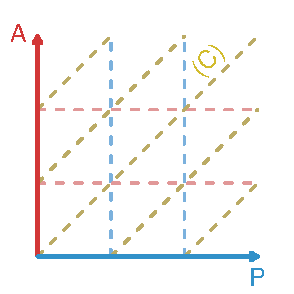
\includegraphics[scale=.5]{Figures/DiagramTable/AP_rt.pdf}
  &
  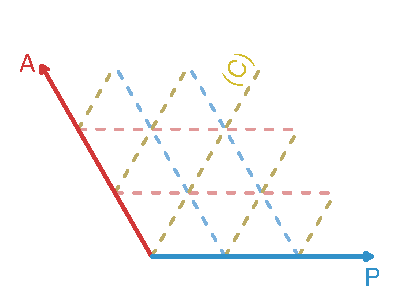
\includegraphics[scale=.5]{Figures/DiagramTable/AP_iso.pdf}
  \\
  %%%% ACp
  $$\begin{aligned}
    &AC(P) \\
    &P = C + A
  \end{aligned}$$ &
  The AC(P) temporal plane is equivalent to the Lexis diagram except birth
  cohort is given and period is derived rather than the other way around. &
  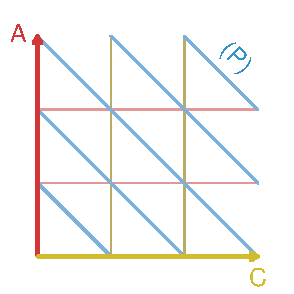
\includegraphics[scale=.5]{Figures/DiagramTable/AC_rt.pdf} & 
  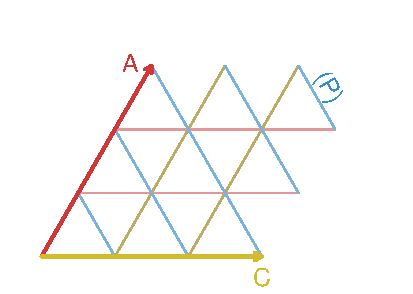
\includegraphics[scale=.5]{Figures/DiagramTable/AC_iso.pdf}  \\
  %%%% CPa
  $$\begin{aligned}
    &CP(A) \\
    &A = P - C
  \end{aligned}$$ &
  The CP(A) temporal plane is equivalent to the Lexis diagram except birth
  cohorts are given and age is derived rather than the other way around. &
  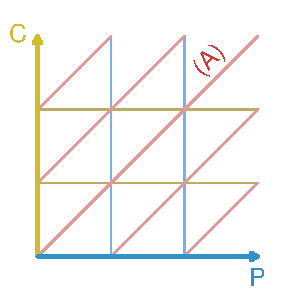
\includegraphics[scale=.5]{Figures/DiagramTable/CP_rt.pdf} & 
  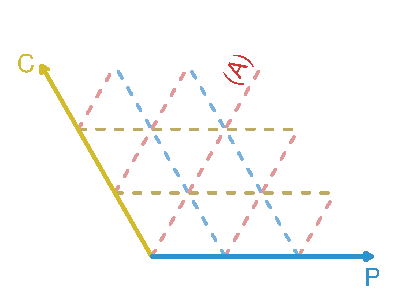
\includegraphics[scale=.5]{Figures/DiagramTable/CP_iso.pdf}  \\
  \midrule
  %%%%%%%%%%%%%%%%%%%%%%%%%%%%%%%%%%%%%%%%%%%%%%%%%%%%%%%%%%%%%%%%%%%%%%%%%%%%%
  \multicolumn{4}{c}{\textsc{Variants of TPD}} \\
  \midrule
  %%%% TPd
  $$\begin{aligned}
    &TP(D) \\
    &D = P + T
  \end{aligned}$$ &
  Helen had 30 years of life left (T) in 1971 (P) and therefore belonged to the 2001 death cohort (D) &
  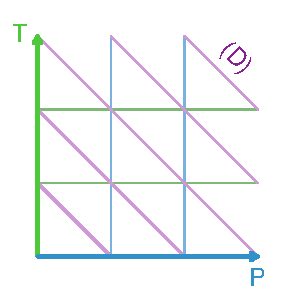
\includegraphics[scale=.5]{Figures/DiagramTable/TP_rt.pdf} &
  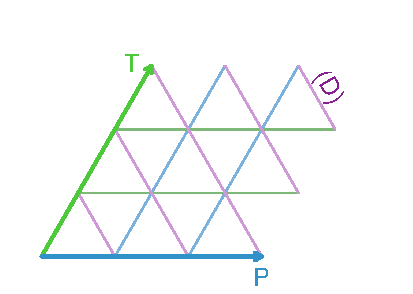
\includegraphics[scale=.5]{Figures/DiagramTable/TP_iso.pdf}  \\
  %%%% PDt
  $$\begin{aligned}
    &PD(T) \\
    &T = D - P
  \end{aligned}$$ &
  Mindel died in 1973 (D). In 1953 (P) she had 20 years left to live (T). &
  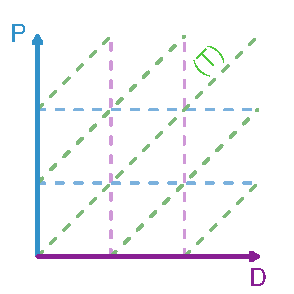
\includegraphics[scale=.5]{Figures/DiagramTable/PD_rt.pdf} &
  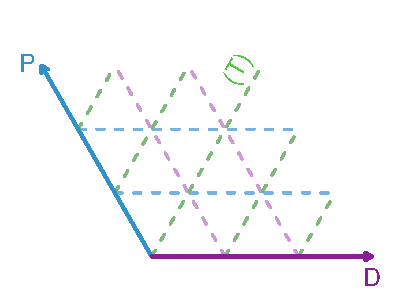
\includegraphics[scale=.5]{Figures/DiagramTable/PD_iso.pdf}  \\
  %%%% TDp
  $$\begin{aligned}
    &TD(P) \\
    &P = D - T
  \end{aligned}$$ &
  Irene died in 1974 (D). When she had 30 remaining years of life (T) the year must have been 1944 (P). &
  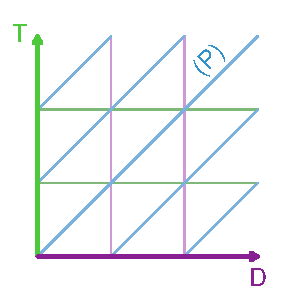
\includegraphics[scale=.5]{Figures/DiagramTable/TD_rt.pdf} &
  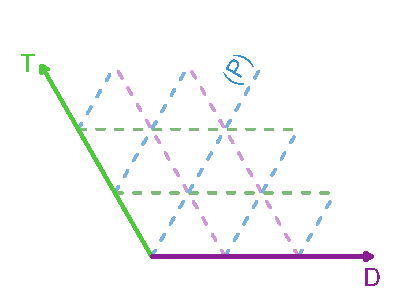
\includegraphics[scale=.5]{Figures/DiagramTable/TD_iso.pdf}  \\
  \midrule
  %%%%%%%%%%%%%%%%%%%%%%%%%%%%%%%%%%%%%%%%%%%%%%%%%%%%%%%%%%%%%%%%%%%%%%%%%%%%%
  \multicolumn{4}{c}{\textsc{Variants of TAL}} \\
  \midrule
  %%%% TAl
  $$\begin{aligned}
    &TA(L) \\
    &L = T + A
  \end{aligned}$$ &
  The time already lived and the time still left sum up to the total lifespan. &
  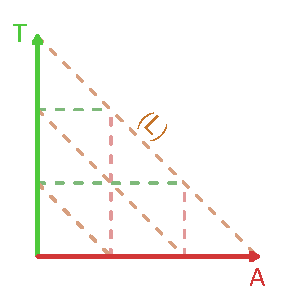
\includegraphics[scale=.5]{Figures/DiagramTable/TA_rt.pdf} &
  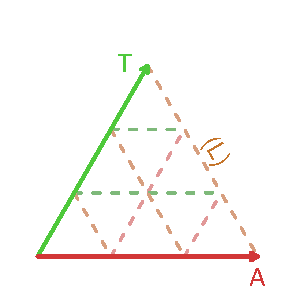
\includegraphics[scale=.5]{Figures/DiagramTable/TA_iso.pdf}  \\
  %%%% TLa
  $$\begin{aligned}
    &TL(A) \\
    &A = L - T
  \end{aligned}$$ &
  Helen lived to the age of 86 (L). When she had 20 years left (T) she must have been 66 (A). &
  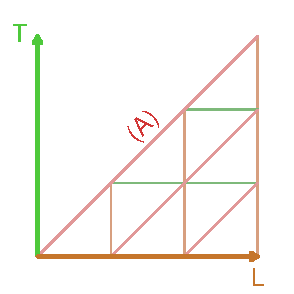
\includegraphics[scale=.5]{Figures/DiagramTable/TL_rt.pdf} &
  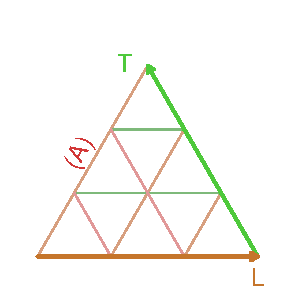
\includegraphics[scale=.5]{Figures/DiagramTable/TL_iso.pdf}  \\
  %%%% ALt
  $$\begin{aligned}
    &AL(T) \\
    &T = A - L
  \end{aligned}$$ &
  Tim is 34 years old (A) and will live to the age of 96 (L), leaving him 62 years (T) to settle affairs. &
  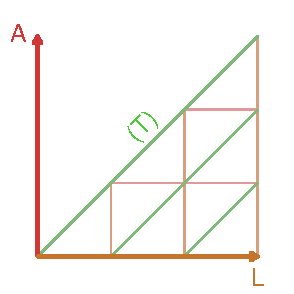
\includegraphics[scale=.5]{Figures/DiagramTable/AL_rt.pdf} &
  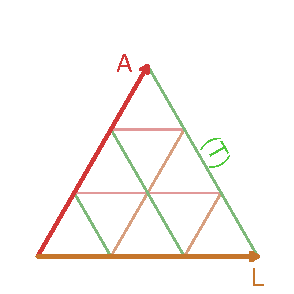
\includegraphics[scale=.5]{Figures/DiagramTable/AL_iso.pdf}  \\
  \midrule
  %%%%%%%%%%%%%%%%%%%%%%%%%%%%%%%%%%%%%%%%%%%%%%%%%%%%%%%%%%%%%%%%%%%%%%%%%%%%%
  \multicolumn{4}{c}{\textsc{Variants of LCD}} \\
  \midrule
  %%%% LCd
  $$\begin{aligned}
    &LC(D) \\
    &D = C + L
  \end{aligned}$$ &
  \`{A}ngels was born in 1940 (C) and she lived to be 64 (L), implying an
  untimely death in 2004 (D) &
  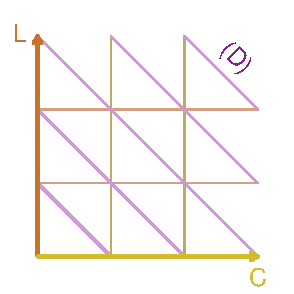
\includegraphics[scale=.5]{Figures/DiagramTable/LC_rt.pdf} &
  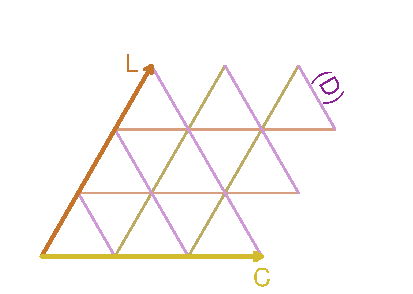
\includegraphics[scale=.5]{Figures/DiagramTable/LC_iso.pdf}  \\
  %%%% CDl
  $$\begin{aligned}
    &CD(L) \\
    &L = D - C
  \end{aligned}$$ &
  Pascal was born in 1893 (C) and died in 1964 (D), implying a lifespan of 71 (L), or so. &
  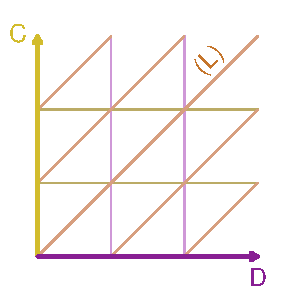
\includegraphics[scale=.5]{Figures/DiagramTable/CD_rt.pdf} &
  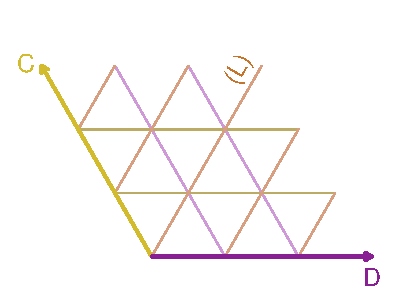
\includegraphics[scale=.5]{Figures/DiagramTable/CD_iso.pdf}  \\
  %%%% LDc
  $$\begin{aligned}
    &LD(C) \\
    &C = D - L
  \end{aligned}$$ &
  Margaret died in Dec., 1995 (D) with a completed lifespan of 96 (L), putting her birth year in 1900 (C). &
  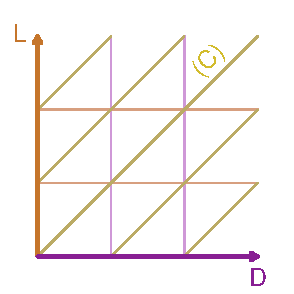
\includegraphics[scale=.5]{Figures/DiagramTable/LD_rt.pdf} &
  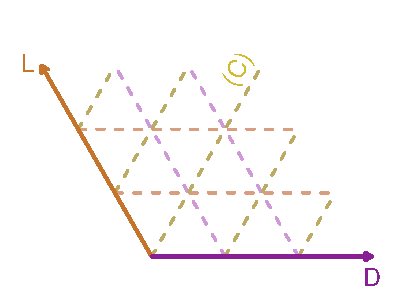
\includegraphics[scale=.5]{Figures/DiagramTable/LD_iso.pdf}  \\
  \midrule
  %%%%%%%%%%%%%%%%%%%%%%%%%%%%%%%%%%%%%%%%%%%%%%%%%%%%%%%%%%%%%%%%%%%%%%%%%%%%%
  \multicolumn{4}{c}{\textsc{The Uninformative Dyads}} \\
  \midrule
  %%%% LP
  LP(-) &
  The LP plane is \emph{non-informative}. No additional measures can be derived knowing just lifespan and period. &
  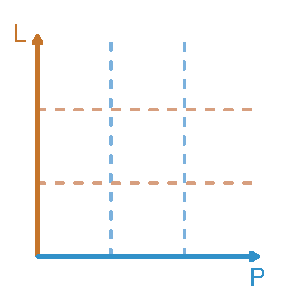
\includegraphics[scale=.5]{Figures/DiagramTable/LP_rt.pdf} &
  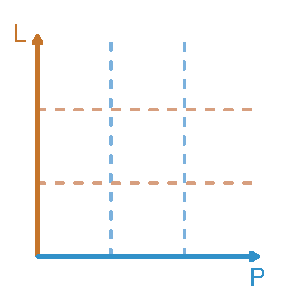
\includegraphics[scale=.5]{Figures/DiagramTable/LP_rt.pdf} \\
  %%%% CT
  CT(-) &
  The CT plane is \emph{non-informative}. No additional measures can be derived knowing just cohort and thanatological age. &
  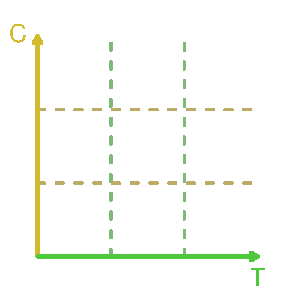
\includegraphics[scale=.5]{Figures/DiagramTable/CT_rt.pdf} &
  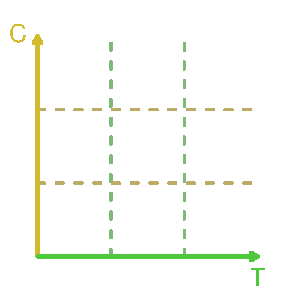
\includegraphics[scale=.5]{Figures/DiagramTable/CT_rt.pdf} \\
  %%%% AD
  AD(-) &
  The AD plane is \emph{non-informative}. No additional measures can be derived
  knowing just death cohort and age. & 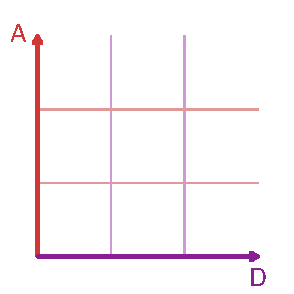
\includegraphics[scale=.5]{Figures/DiagramTable/AD_rt.pdf} &
  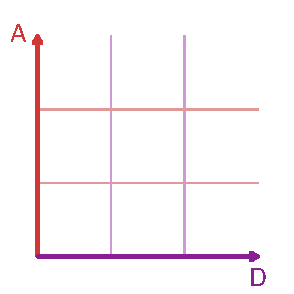
\includegraphics[scale=.5]{Figures/DiagramTable/AD_rt.pdf}  \\
  \bottomrule
\end{longtable}

Most of what we know about how rates change over age and time comes
from the very first juxtaposition in Table~\ref{tab:dyads}, AP(C). While
CP(A) and AC(P) are statistically redundant when exact times are used, they
are not fully redundant if based on discrete double-classification of data, as
often provided in aggregated official statistics. Double classified data are
found on the APC diagram in the shape of squares (AP), horizontal parallelograms
(AC) and vertical paralellograms (PC), and
these are commonly used to compute different kinds of demographic
rates and probabilities \citep[][p63]{caselli2005demography}. The other dyadic
juxtapositions (involving the measures T, D, or L) can be considered as either
rare or novel ways of structuring or viewing temporal variation in demography,
and these imply new families of rates and probabilities.

\subsection{The triad identities}
There are $20=\binom{6}{3}$ ways to choose three time indices out of
six, of which four form a triad identity: APC, TPD, TAL, and LCD.
Given the three time measures from any of the
triad identities, one can derive no further time measures. If one selects three
random time indices that do not form any of these four triad identities
($20-4=16$ possibilities), this property does not hold. For instance, in the
triad APT, age and period are not sufficient to determine thanatological age.
Given the triad APT one can however derive the remaining three time
measures.%\footnote{We return to the case of APT and similar constructs in later sections.}

%Visualizations of data structured by any dyad belonging to a triad identity
%are inherently richer in information than are juxtapositions of uninformative
%dyads. 
Triad identities are more meaningful than uninformative dyads. This
is so even in the absence of data, due to the underlying relationship between
measures. Each of the triad identities can accommodate some version of a
lifeline, for instance. In the following, we therefore lay out the four primary
diagrams that belong to the triad identities. The question of which diagram
mapping is relevant to a given demographic phenomena is a function of
patterns in the data. The best diagram is the one that captures all meaningful
variation in the data. If APC highlights meaningful variation in a phenomenon,
then its representation as such is useful. The same holds for the other
identities. With each diagram in following we comment or speculate on its
potential uses.

\subsubsection{APC: Chronological age, period, and birth cohort}%\tgh{APC}}
\FloatBarrier
The so-called Lexis diagram has long been used in demography as a conceptual
tool for structuring data, observations, and rate estimation, as inspiration for work
on statistical identification, and as the coordinate basis of contemporary
Lexis-surfaces.\footnote{Some prefer the term Lexis \textit{surface}, while
others prefer to call them contour maps, heatmaps, or stereograms.}
Since the Lexis diagram could have been named for others
\citep{keiding2011age, vandeschrick2001lexis}, and since we compare with other
temporal configurations, let us refer to it as the APC diagram, as seen in
Figs.~\ref{fig:APCrt} and~\ref{fig:APCeq}. 

\begin{figure}[h!] 
\caption{An APC diagram in two projections.}
\label{fig:APC}
\centering
\begin{subfigure}{1.1\textwidth}
\caption{Cartesian}
\vspace{-5em}
\label{fig:APCrt}
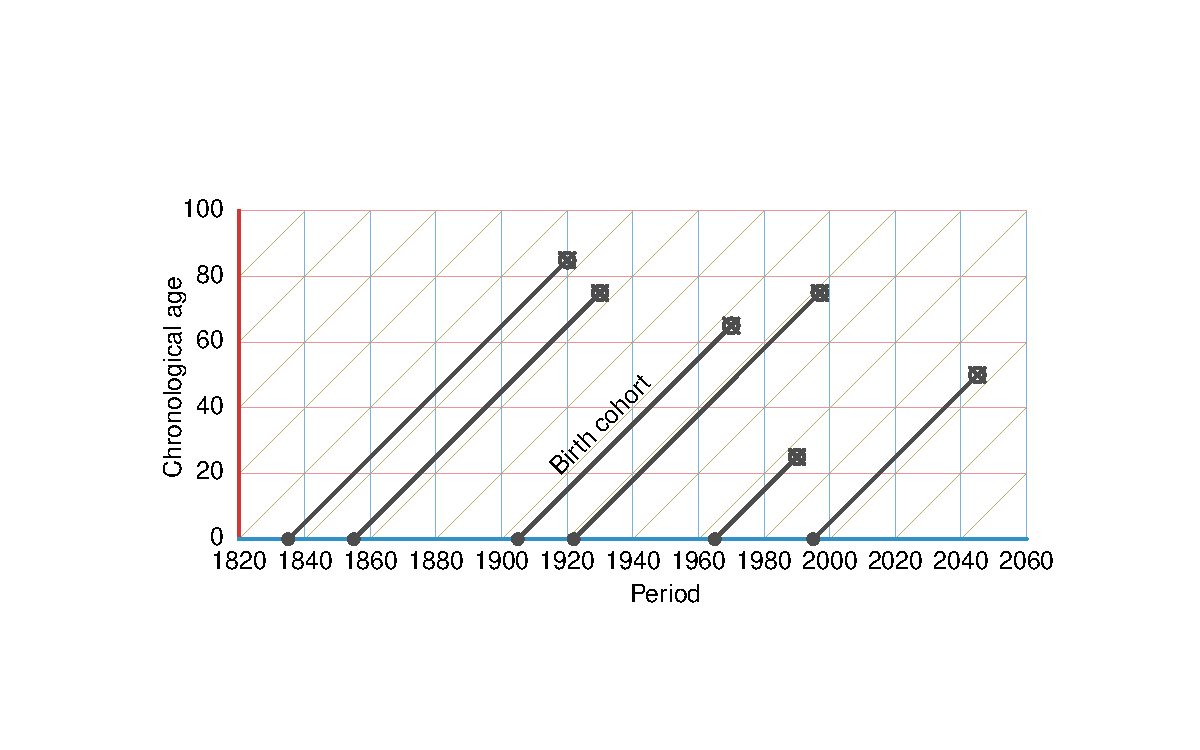
\includegraphics[scale=0.8]{Figures/APCrt.pdf}
\end{subfigure}
\\\vspace{-2em}
\begin{subfigure}{1.1\textwidth}
\caption{Isotropic}
\vspace{-6em}
\label{fig:APCeq}
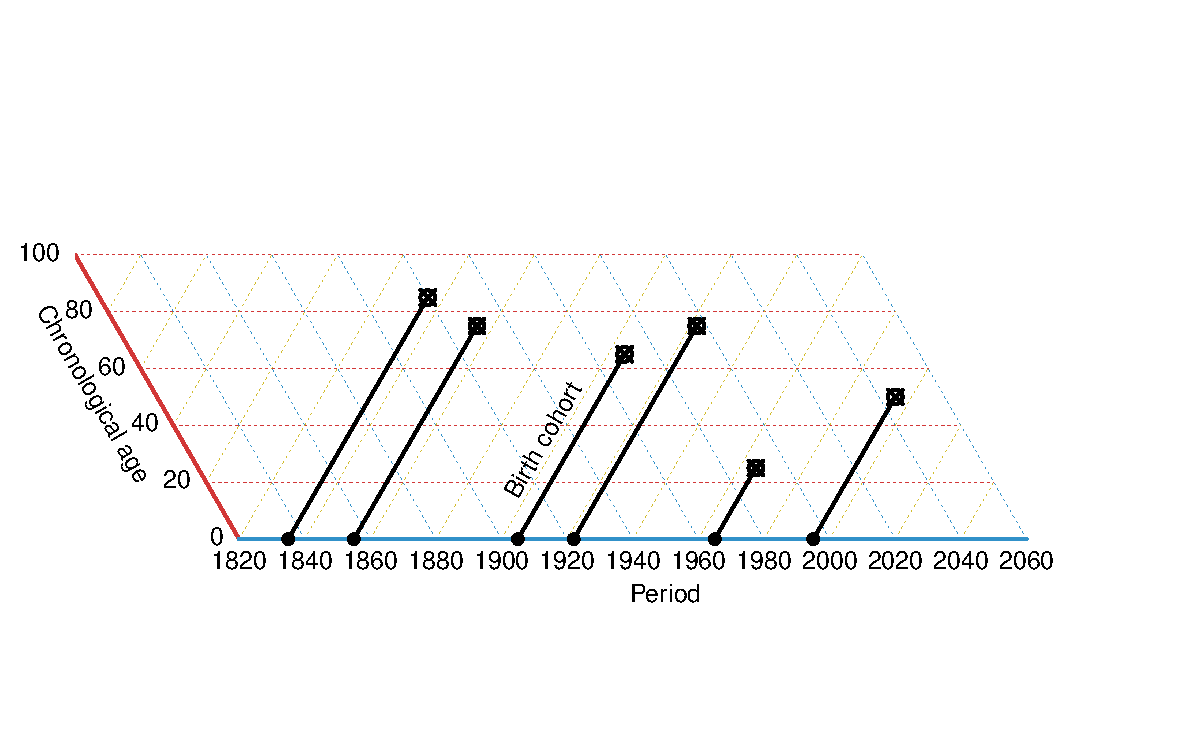
\includegraphics[scale=0.8]{Figures/APCeq.pdf}
\end{subfigure}
\end{figure}

The APC diagram in Figure~\ref{fig:APCrt} represents years lived on the $y$
axis, calendar years on the $x$ axis, and birth cohorts as the right-ascending
diagonals. This is the most common of several possible configurations
of the APC dimensions. Individual lifelines (black) are aligned in the birth
cohort direction, starting with birth (filled circle) at chronological age zero, and death
(circled x). Any APC surface can be interpreted along each of these
three dimensions of temporal structure. 

\FloatBarrier
\subsubsection{TPD: thanatological age, period, and death cohort}%\tgh{TPD}}

Thanatological age (T), period (P) and death cohort (D) form a coordinate system
best imagined as the inverse of APC. One may take the same individuals
represented in Figure~\ref{fig:APC} and group them by death cohorts (D) instead
of birth cohorts (C). Lifelines then descend such that all
endpoints align to thanatological age 0, creating the diagram in Figure 2 in which individuals dying at different ages but in the same time period are grouped together.
To our knowledge, the TPD diagram has only appeared once in the literature, as
a didactic aid in a proof of symmetry between chronological and thanatological
age structure in discrete stationary populations \citep{villavicencioRiffeSymmetires2016}. TPD
diagrams may also be useful to arrange events or durations that are logically
aligned (or may only be aligned) by time of termination. It may be reasonable to
align on termination in cases where this brings preceding patterns of
variation into focus.

\begin{figure}[h!] 
\caption{A TPD diagram in two projections.}
\label{fig:TPD}
\centering
\begin{subfigure}{1.1\textwidth}
\caption{Cartesian}
\vspace{-5em}
\label{fig:TPDrt}
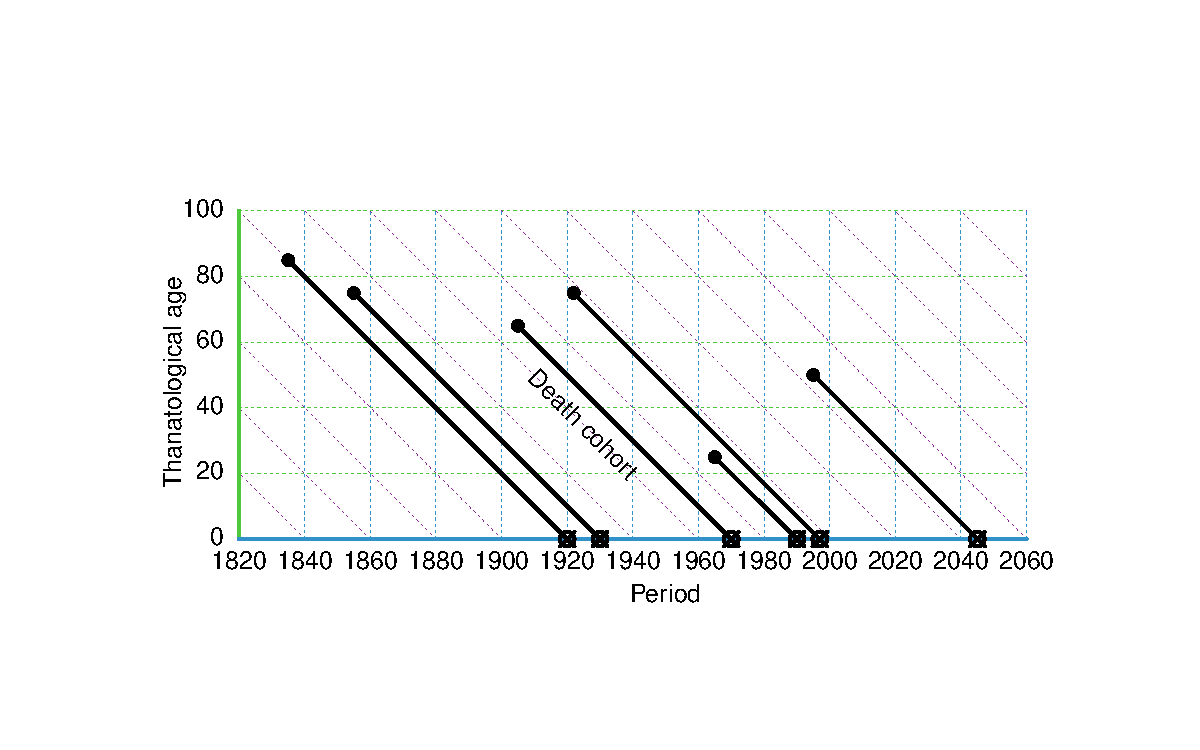
\includegraphics[scale=0.8]{Figures/TPDrt.pdf}
\end{subfigure}
\\\vspace{-2em}
\begin{subfigure}{1.1\textwidth}
\caption{Isotropic}
\vspace{-6em}
\label{fig:TPDeq}
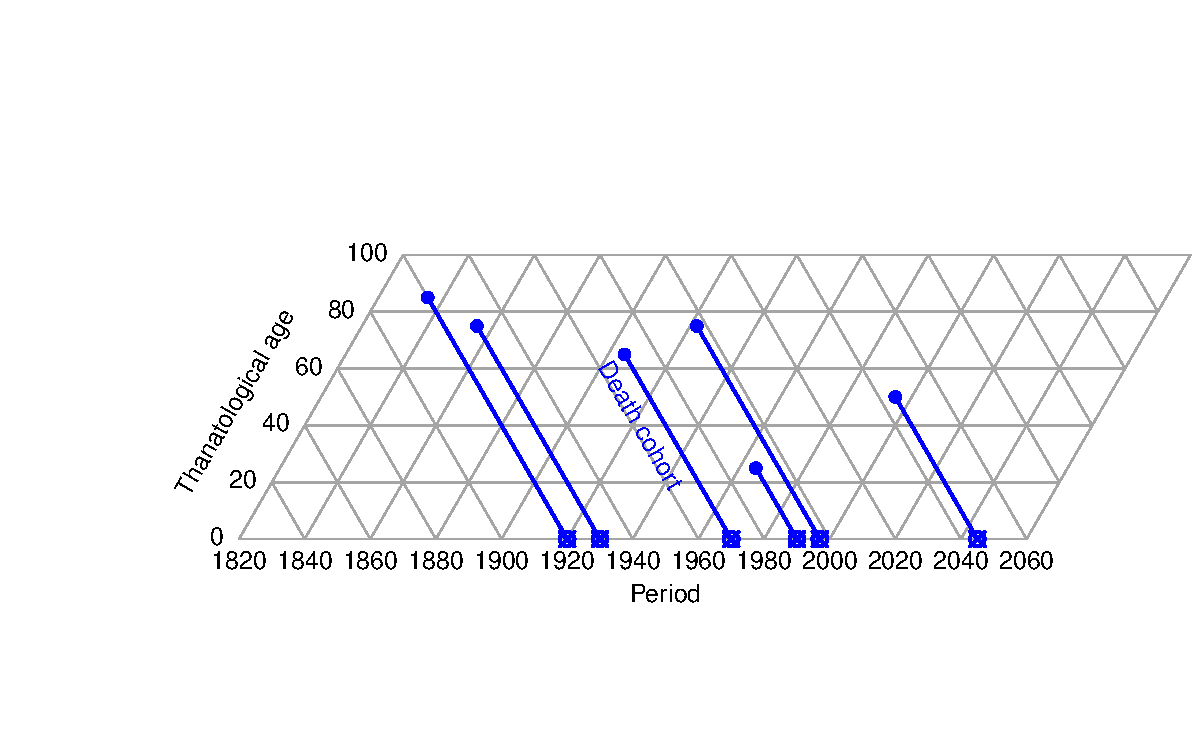
\includegraphics[scale=0.8]{Figures/TPDeq.pdf}
\end{subfigure}
\end{figure} 

There are several examples of analysis of this kind of
data, usually stemming from a lack of information on chronological age. This is
the case, for instance, in biodemographic studies in which wild animals with unknown
ages are captured and then followed-up until death
\citep{Muller2004,Muller2007}, but it can be generalized to other kinds of human
and non-human demographic data with a similar structure. For example, in the
Barcelona Historical Marriage Database, which collects information about
marriage licenses of Barcelona (Spain) from the mid-\nth{15} century until the
early \nth{20} century, individuals are first identified in their marriage
record and then followed-up, but no information is available about dates of
birth or marriage \citep{villavicencio2015lifespans}.
We speculate that TPD diagrams could also be used in biomedical studies
for the representation of lifelines preceding deaths from infectious or acquired conditions, when the time of infection or acquisition remains unknown.


\FloatBarrier
\subsubsection{TAL: Thanatological age, chronological age, and
lifespan}%\tgh{ATL}}
\FloatBarrier  
TAL is an appropriate coordinate
system to examine variation in processes that vary over the lifecourse.
More precisely, the TAL plane can highlight variation that is related to time
since birth, time until death, length of life, and their combinations. These
key aspects of demographic time are compressed to chronological age only in the
APC perspective, which can blend out meaningful variation. Since the lifecourse belongs to the cohort perspective, it is best to think of the TAL plane as belonging to some particular birth cohort. Alternatively, a TAL triangle may be taken as a cross-section through the period dimension, a sort of synthetic TAL plane. To our knowledge, the TAL diagram has only appeared once in the literature, in an exploration and classification of late-life health
conditions \citep{riffe2015ttd}. The TAL diagram in Fig.~\ref{fig:TAL} contains
no indication of period or cohorts, as calendar time is blended out in this
diagram.
The lifelines depicted are identical to those shown in APC Fig.~\ref{fig:APC} and TPD Fig.~\ref{fig:TPD}.\footnote{The prior figures contained six lifelines each, but since two of them were of equal length (75), they are overlapped in
Fig.~\ref{fig:TAL} and appear to be five.} The TAL diagram is useful for
characterizing patterns of prevalence of health conditions. We speculate
that data structured and aligned in this way may yield hitherto undescribed
patterns in other contexts, such as smaller event-history time scales, or
patterns of growth or reproduction in non-human species.

\begin{figure}[h!] 
\caption{A TAL diagram in two projections.}
\label{fig:TAL}
\centering
\makebox[\textwidth][c]{
\begin{subfigure}{.48\textwidth}
\centering
\caption{Cartesian}
\label{fig:TALrt}
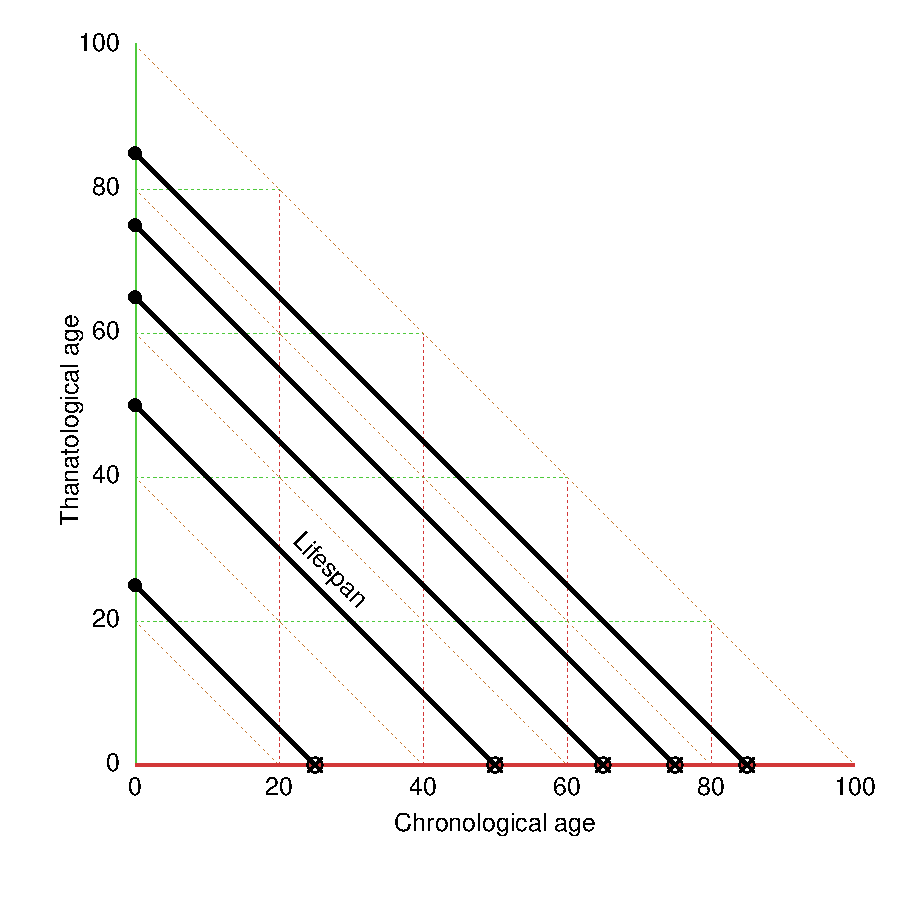
\includegraphics[scale=0.55]{Figures/TALrt.pdf}
\end{subfigure}
~~~~~
\begin{subfigure}{.48\textwidth}
\centering
\caption{Isotropic}
\label{fig:TALeq}
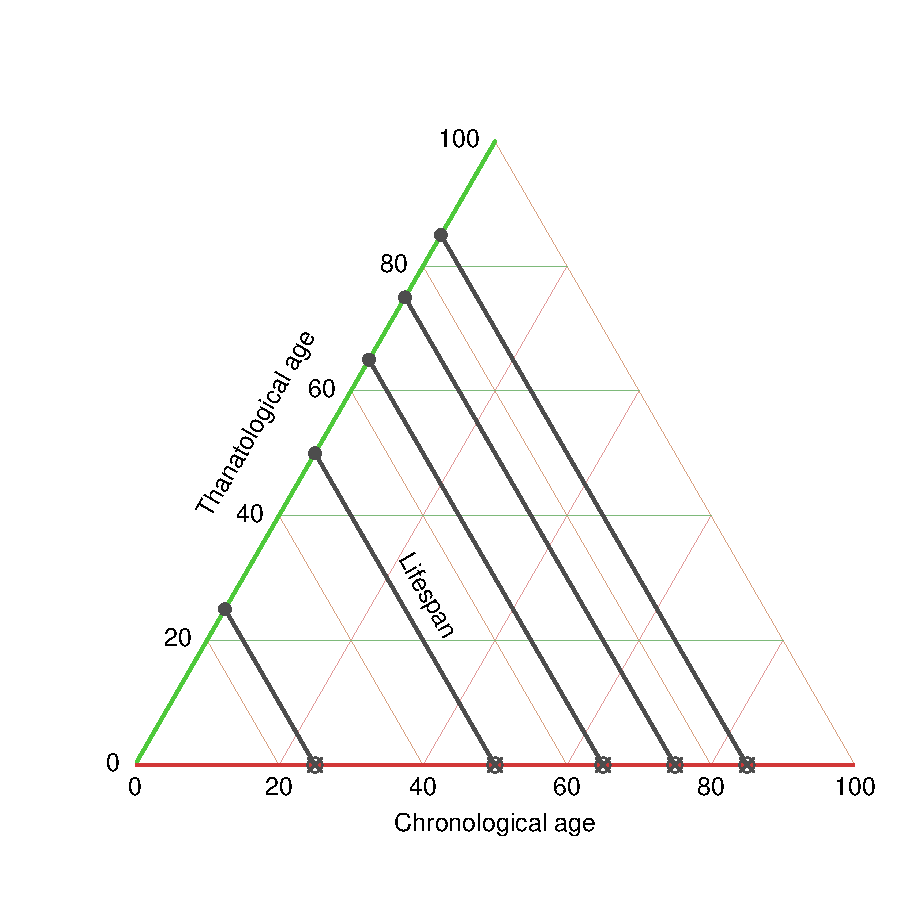
\includegraphics[scale=0.55]{Figures/TALeq.pdf}
\end{subfigure}
}
\end{figure} 

\FloatBarrier
\subsubsection{LCD: Lifespan, birth cohort, and death cohort}%\tgh{CDL}}
\FloatBarrier

The LCD diagram completes our set of identities. It consists in an identity
between lifespans, birth cohorts, and death cohorts. In Fig.~\ref{fig:LCDrt},
lifespans are indexed by the $y$-axis, while birth cohorts are indexed by the $x$-axis, and death cohorts
are found in rightward-descending diagonals. To structure data on these three
time measures implies excluding time-varying information over the lifecourse.
An individual
only ever has one lifespan, one birth cohort, and one death cohort, such that
the LCD coordinates of an individual are constant throughout life.
Individuals can therefore be identified with points only in the LCD diagram,
rather than lifelines. In Fig.~\ref{fig:LCD}, the same six individuals from
previous diagram figures are represented with crossed circles.

\begin{figure}[h!] 
\caption{An LCD diagram in two projections.}
\label{fig:LCD}
\centering
\begin{subfigure}{1.1\textwidth}
\caption{Cartesian}
\vspace{-5em}
\label{fig:LCDrt}
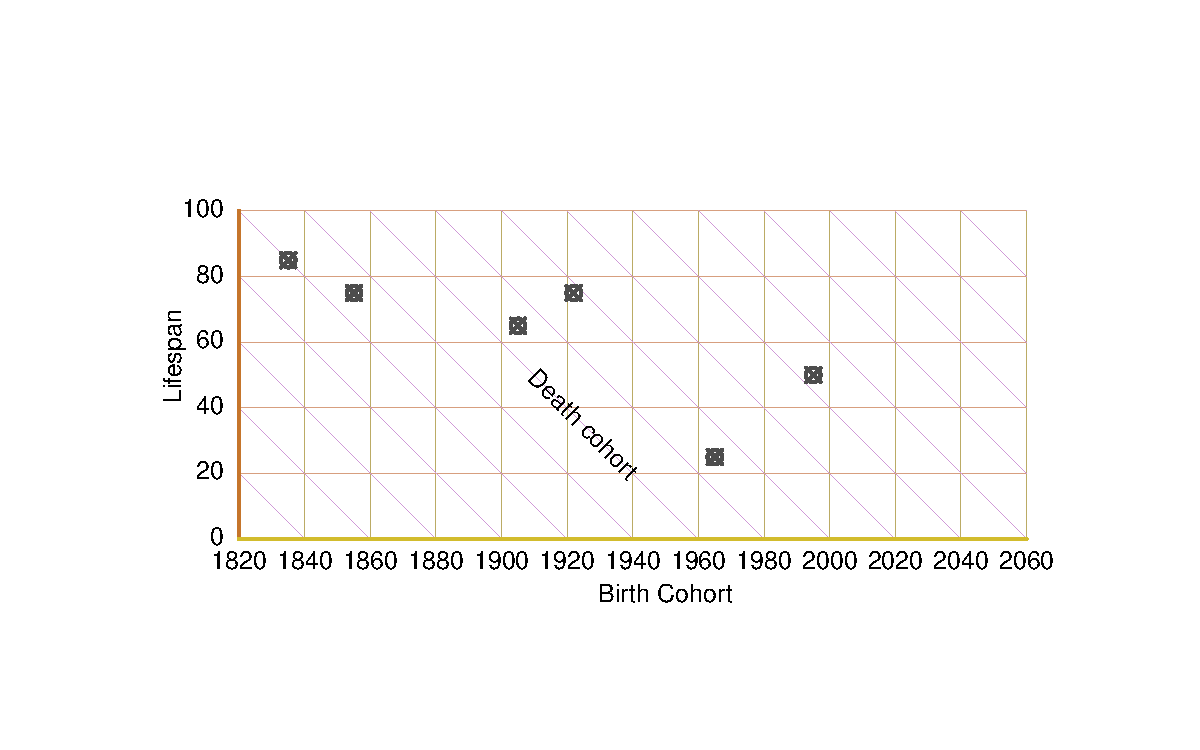
\includegraphics[scale=0.8]{Figures/LCDrt.pdf}
\end{subfigure}
\\\vspace{-2em}
\begin{subfigure}{1.1\textwidth}
\caption{Isotropic}
\vspace{-6em}
\label{fig:LCDeq}
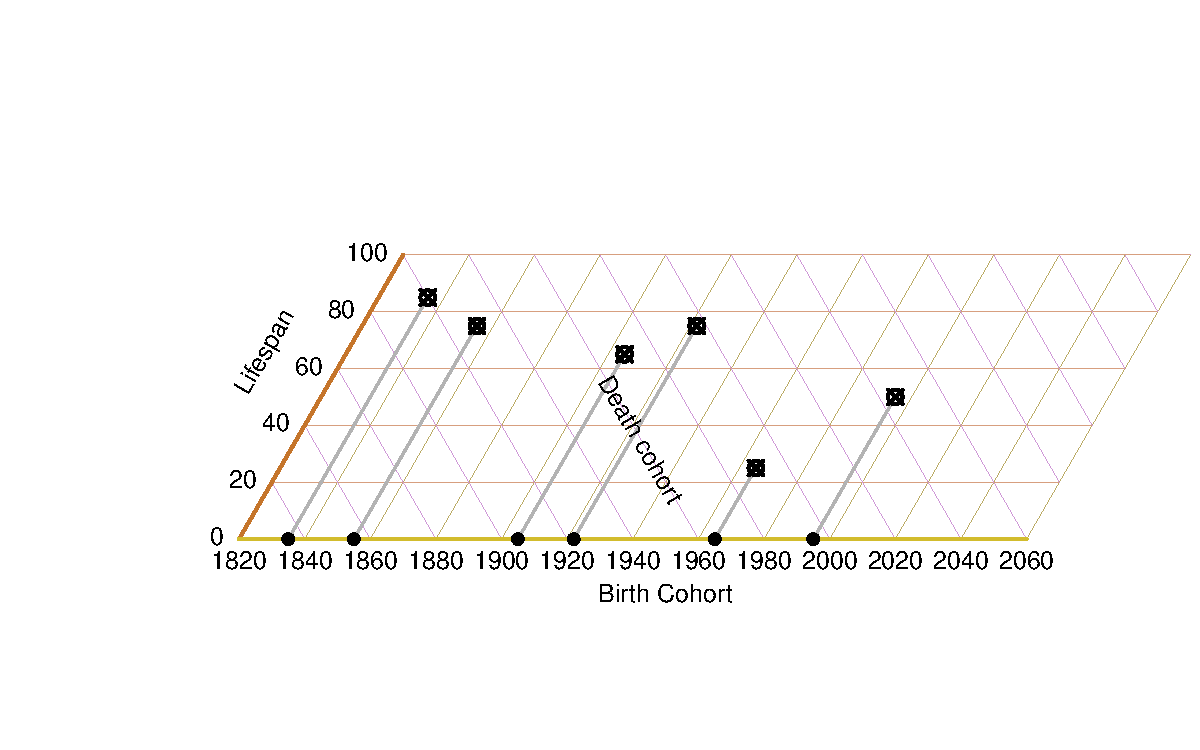
\includegraphics[scale=0.8]{Figures/LCDeq.pdf}
\end{subfigure}
\end{figure} 

We
recommend this mapping for plotting surfaces of values that vary over time by year of birth or death and that vary by lifespan, e.g., that are cumulative or
static over the lifecourse. Imagine an LCD surface of cumulative lifecourse
consumptive surplus or deficit, or anything else that might vary by lifespan and
moment of birth or death, such as children ever born, years of retirement, the
size of trees or other aspects of forestry, populations of buildings in large
cities, and so forth. \citet{lexis1875einleitung} describes an analogous
relationship between marriage cohort, separation cohort, and duration of
marriage.

\subsubsection{Relationships between the diagrams}
Since demographic time measures themselves depend on the demographic events of
fertility and mortality, it stands to reason that fertility and mortality also
link the different diagrams. In a loose sense, the LCD diagram has a
special dual in the case of an APC surface of mortality. Age at death is equal
to lifespan ($A=L$), period is equal to death cohort ($P=D$), and birth cohort
(C) is just the same in the event of death. These two surfaces are exactly
equivalent in the case of death counts or densities, since in either case
quantities are represented with points, the endpoint of life for which this
equivalence holds. For any other demographic measure, however, the LCD diagram
is distinct from APC. APC fertility surfaces are in this way very different from
APC mortality surfaces, as the former represent events or characteristics over
the ages in which they occur, allowing for the represention of
durations and repetitions.
Further, a fertility surface in TPD coordinates
again finds an approximate dual in the APC mortality surface. This works
because birth marks the starting point of the lifeline which is otherwise
missing in TPD coordinates, whereas death marks the endpoint of a lifeline,
which is otherwise missing from APC coordinates. This relationship is exact in
the special case of a stationary population. Further reflection may
reveal other such dualities.

\FloatBarrier
\section{A tetrahedron relates the six time indices.}
Each of the four triad identities may be thought of as a
two-dimensional plane fully defined by any two of its three constituent time
indices.
In this case, we may imagine any of the excluded time measures as capable of
providing depth, a potential $z$-coordinate, for the sake of a mental image.
Having a non-redundant third dimension implies a multitude of parallel planes
for the given triad identity, each plane belonging to a unique value of the
third time dimension. Any of the identities can be extended in this way to fill a space. A space derived by
extending any of the triad identities into its lacking dimension implies each of
the other triad identities, making a total of six time indices. In essence, the
four triad identities may be thought of as the four faces of a
tetrahedron. If an additional time measure is added to any face (triad
identity), the six demographic time indices can be derived, matching the six edges of the tetrahedron. This three-dimensional construct unifies the six indices of demographic time, and is the subject of this paper.

Let us first more rigorously define the previously-mentioned tetrahedron.
Luckily, the edges and vertices of a tetrahedron are easily rendered in a
two-dimensional graph, as seen in Fig.~\ref{fig:tet}, with vertices labeled
in black and the six time indices colored following the pattern from
Table~\ref{tab:dyads}. The tetrahedron is composed with the APC plane at the
base and vertex 4 on top. The same graph could be composed in four basic
ways, depending on which identity forms the base.
%The reader may also imagine this graph as a transparent 3d object, in which
% case the four faces become apparent. There are two intuitive ways to imagine the graph as 3d, either the vertex 4 is on top, and we gaze from a bird's-eye-view, or the vertex 4 is in the back, behind the other three vertices. Assume we gaze from the top, for the sake of description.\footnote{The same graph
%could be composed in four basic ways, depending on which triad-identity face
%forms the base.
%These are given in an appendix.} 

\begin{figure}[h!]
\centering
\caption{Graph of tetrahedron, with edges labeled by the six demographic time
indices. The APC plane is at the base, and vertex four on top.}
\label{fig:tet}
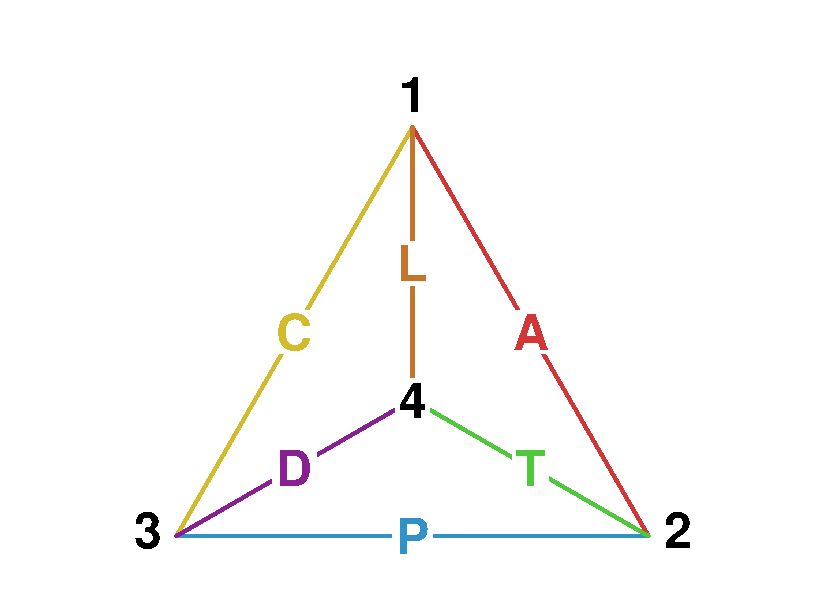
\includegraphics[scale=.8]{Figures/TetraHedronVerticesEdges.pdf}
\end{figure}

The edges APC at the base define the much-studied APC plane. If the only
information we have is chronological age, period, and birth cohort (or just two
of these), then we have no access to the vertex 4. Each of the faces of the
tetrahedron has this quality. The South face TPD has no access to 1.
The Northeast face, TAL has no connection to 3, and the Northwest face
LCD lacks a connection to 2. The four triad identities that make up the faces of
the tetrahedron are stuck in ``flatland'' and do not yield the full 3d
space. However, the 16 other possible combinations of three time indices will
recreate the full tetrahedron (hexad identity).

% PV: I suggest to replace the following paragraph, or at least to introduce
% this geometrical perspective somewhere in the text

%   TR: OK, I've commented it out. The removed paragraph sounds more like advice
%       on how to manually find all 20-16-12 triads without too much mental
%       labor. Maybe worth an appendix?
% TR: the vector description is probably more rigorous, so let's go with it.
%     We'll put some effort later into making it understandable for avg
%     demographers.

%\sout{For example, say we are at vertex \vt{1}, and we therefore have
%information on year of birth C, completed lifespan L, and
%chronological age A (see Figure~\ref{fig:tet4vert1}). Clearly, A and
%C imply P ($C+A=P$).
%A and L imply T ($L-A=T$). Finally, C and
%L imply D ($C+L=D$), and we have the full hexad
%identity. In the tetrahedron graph, we have three edges that connect to the
%four vertices. This is the essential property of a fully informed triad.
%It is easily verified that each vertex has this property.
%However, there are twelve other sets of three that also have this property. To
% locate these ``hidden'' triads, first note that each index has an
%opposite index, with which it shares no information. These pairs are
%A-D, L-P, and C-T, and can be found in Figure~\ref{fig:tet} as
%the three sets of perpendicular edges. Each of these pairs can be completed
% into a `fully-informed'' triad by the addition of any of the other four indices
%(thereby connecting the edges). Doing so for each of the opposite pairs will
%yield the remaining twelve triads.}

\subsection{A geometrical analogy}
A geometrical analogy is pertinent at this point. Any pair of intersecting edges
of the tetrahedron may be interpreted as two vectors $\vec{u}$ and $\vec{v}$
that determine a 2-dimensional plane in a Cartesian 3-dimensional
space ($\mathbb{R}^3$).\footnote{A 2d plane in a 3d space is determined by two linearly independent
vectors (with different direction) and a point, but the inclusion of a point is not
necessary for the intuitive analogy that we describe here.} Therefore, any third
vector $\vec{w}$ of that plane can be expressed as a linear combination of
$\vec{u}$ and $\vec{v}$ (formally, $\vec{w}=\alpha\vec{u}+\beta\vec{v}$ for some $\alpha, \beta \in \mathbb{R}$), which is usually
described by saying that $\vec{w}$ is linearly dependent on $\vec{u}$ and
$\vec{v}$.
A similar property can be derived from the information contained in the
tetrahedron: $A=P-C$ is a linear combination of C and P and it ``depends''
on them because they all belong to the same APC plane. Analogously, $P=C+A$
``depends'' on C and A, and $C=P-A$ ``depends'' on P and A. Given that the faces of the tetrahedron represent the triad identities, any pair of intersecting edges has the same property: The third edge located in the same face of the tetrahedron can be determined by the first two by a simple linear relationship.

% code given in R/TetraCombos.R, lines 70-95
% PV: already created the new figure
%\begin{figure}[h!]
%\centering
%\caption{Graph of tetrahedron, edges belonging to the APC face highlighted.}
%\label{fig:tet4vert1}
%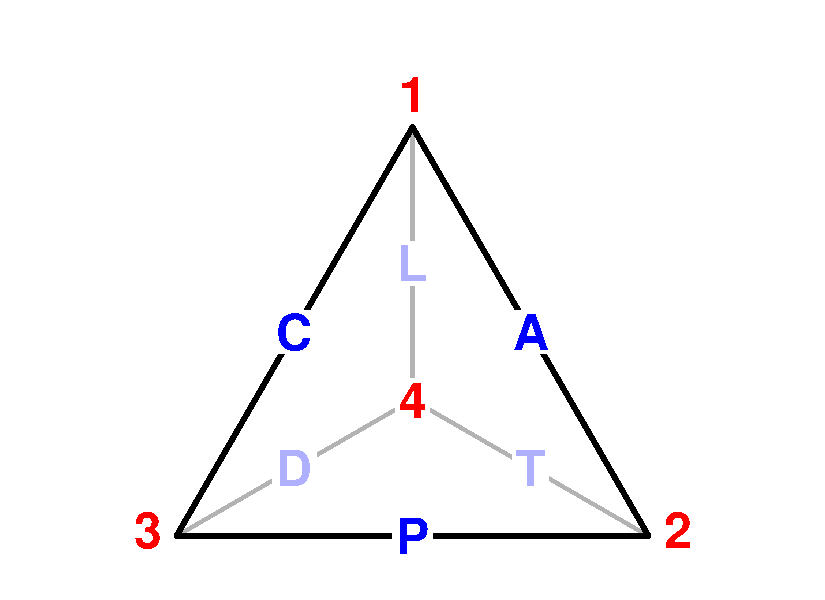
\includegraphics[scale=1]{Figures/tet4vert1New.pdf}
%\end{figure}
%\noindent 

Once a 2d-plane is defined in $\mathbb{R}^3$, an additional vector may be sufficient to cover a
3d-space. Nonetheless, this third vector needs to be linearly independent
of any pair of vectors of the 2d plane---that is, it cannot be expressed as a
linear combination of any two vectors on that plane. Again, an analogous
property can be observed in the tetrahedron: Say we only have information about
the indices of the APC plane; A, C and P are not sufficient to determine a thanatological age T, death cohort D, or lifespan L (the three indices that do not belong to the APC plane). So, T, D and L are ``independent'' of the overall information that can be extracted from the APC plane. However, if two of the three constituent time indices of the APC plane are known (the third one would be unnecessary as it could be derived from the other two), the additional information provided by any of the three ``independent'' indices T, D or L would be sufficient to cover the whole tetrahedron. For example, suppose we have information about thanatological age T in addition to C and P, then $A=P-C$, $D=P+T$ and $L=T+A=T+P-C=D-C$. 

Hence, as with vectors in a 3d space, any
triad of indices that are independent of each other---that is, none of them can
be expressed as the sum or the difference of the other two---generates a full
hexad identity or, using an analogous terminology, covers the whole ``space'' of
demographic indices presented here. Graphically, this is equivalent to
choosing any combination of three indices that do not belong to the same face
of the tetrahedron.%, i.e., that do not form one of the four triad identities
%represented in Table~\ref{tab:triadids}.

% TR: moved
%There are $20=\binom{6}{3}$ ways to choose three time indices out of
%six, of which four form a triad identity: APC, TPD, TAL, and LCD.
%Given the three time measures from any of the
%triad identities, one can derive no further time measures. If one selects three
%random time indices that do not form any of these four triad identities
%($20-4=16$ possibilities), this property does not hold. For instance, in the
%triad APT, age and period are not sufficient to determine thanatological age.
%Given the triad APT one can however derive the remaining three time measures.

%\begin{table}[h]
%\centering
%\caption{The four triad identities on the tetrahedron (same orientation)}
%\label{tab:triadids}
%\begin{tabular}{cccc}
%APC & TPD & ATL & CDL\\
%\tg{APC} & \tg{TPD} & \tg{ATL} & \tg{CDL}
%\end{tabular}
%\end{table}
%When graphed in this way, it is clearer that every triad identity surface lacks
% a connection to the opposite vertex of the tetrahedron.
\subsection{The informative triads}
Table~\ref{tab:set3} gives the full set of 16 index-triads that are
informative in the sense that each of them implies the full hexad identity.
Practically, this means that if a given dataset contains variables in one of
the combinations displayed in Table~\ref{tab:set3} that the entire
temporal relationship is available to the researcher.

Note that the 12 possible pairs of intersecting edges on the tetrahedron are, in
fact, the informative dyads described in Table~\ref{tab:dyads}, whereas the uninformative dyads LP, CT, and AD are the pairs of opposite edges of the tetrahedron. As discussed, all 12 informative dyads generate one of the four triad identities, but no dyad will generate the hexad
identity since a third ``independent'' time dimension is necessary.
Similarly, any quad of indices is sufficient to complete the hexad identity, as
at least one of them will not belong to the same face of the tetrahedron, but a
triad may be sufficient if its edges do not all belong to the same plane forming
a triad identity.

\begin{table}[h]
\centering
\caption{All triads from which the full tetrahedron is derivable (same
orientation).}
\label{tab:set3}
\begin{tabular}{cccc}
ACD & ACL & ACT & ADL\\
\tg{ACD} & \tg{ACL} & \tg{ACT} & \tg{ADL}\\
ADP & ADT & ALP & APT\\
\tg{ADP} & \tg{ADT} & \tg{ALP} & \tg{APT}\\
CDP & CDT & CLP & CLT\\
\tg{CDP} & \tg{CDT} & \tg{CLP} & \tg{CLT}\\
CPT & DLP & DLT & LPT\\
\tg{CPT} & \tg{DLP} & \tg{DLT} & \tg{LPT}
\end{tabular}
\end{table}

%FloatBarrier
\subsection{The extension of time axes.}
We have said that planes defined by the four triad identities are parallel to
the faces of the the above-described tetrahedron. In imagining this three-dimensional
relationship, we are no longer confined to the extent of the tetrahedron used thus far for orientation. Instead each of its edges extends a
certain distance in either direction, and each face of the tetrahedron
tessellates to fill its plane.
It may therefore help to first consider the extension of each axis (or index).
Some indices have a lower bound of zero and an upper bound set by the maximum
length of life, $\omega$, while others are boundless. A, T, and L
are clearly in the range $[0,\omega]$.\footnote{It's best to imagine some number like 122.45 years, for $\omega$, rather than infinity. This is the longevity record at the time of this writing. Jeanne L. Calment would have had
$T=122.45$ at birth, $A = 122.45$ at death, and $L=122.45$ for
her entire life.} P, C, and D are bounded only by the inception and extinction of
our species, but may be thought of as boundless, or benchmarked
to our earliest and most recent observations for practicality.\footnote{We
explain the choice of the word ``benchmarked''. Say we have a data series that runs from 1751 to 2011, and an upper age
interval of $110+$. Then we could say that P is in the range $[1751,2011]$,
but by another reading, P must range from at least as early as the earliest
C and until at least as late as the latest D. Someone dying at 110 in 1751
had a C of 1640, and an infant born in 2011 that is destined to live to 110
will die in 2121. In this case a P that \textit{contains} the observed
population will extend well before and after the observed data series, even
more so if we take into account that $\omega > 110$.} As an abstraction,
however, the dimension of calendar time in this model is infinite. Of the four
triad identities, only one lacks an unbounded dimension, the TAL. Adding
the absent dimension to TAL therefore makes its 3d extension boundless. In
this way, we may imagine a prism-like construct, where T, A, and L, compose
the faces of a triangular cross-section of the prism, which extends infinitely
``through'' the triangle.
We can think of the TAL triangle passing through time, extending the population
forward to infinity. In this case, the TAL triangle may take either the period
or cohort perspective. 

 \section{Diagram of the hexad identity}
 There are different ways to proportion this three dimensional construct,
of which we only present the isotropric mapping. In an isotropic projection, the
tetrahedron is regular, such that all edges are of the same length, and the
units of each of the six represented time measures are therefore equal. In this
case, the four triad identities map to temporal planes as tessellations of equilateral
triangles, and the four planes are joined together such that each is parallel to
a face from the regular tetrahedron. When the plane parallel to each
respective face is repeated in equal intervals, we have an isotropic 3d space.\footnote{The isotropic space that results from this
framework is known in other disciplines with different
nomenclatures. In geometry, this structure is called the
tetrahedral-octahedral honeycomb, a variety of space-filling tessellation. In
architecture, it is found in the octet truss system. In physics it is called
the isotropic vector matrix. Constructs following this geometry exist in nature,
in other theoretical settings, and in man-made structures.}
Displaying all planes simultaneously creates a very dense and difficult-to-read
diagram. We opt to delineate the space using particular planes and
intersections.

Fig.~\ref{fig:apctTAL} gives a view of a demographic
time diagram that corresponds to the hexad identity, where birth-cohort TAL
cross-sectional planes are placed in sequence in a perspective drawing.\footnote{The coordinates used to render Figure~\ref{fig:apctTAL} are isotropic.
However, there are no 60$^\circ$ angles in this figure due to the use of
parallax and an indirect viewing angle in this rendering for the sake of
increased legibility.} The most recent TAL plane, for the year 2000, is placed
in the front, whereas past TAL planes are stacked behind it, highlighted in
25-year intervals. The left edge of the frontmost TAL plane is labelled as an
axis for thanatological age, although the same tick marks also serve for
completed lifespan.
The base of this figure is the APC plane, drawn for thanatological age 0.
Each of the TAL planes sits atop a single birth cohort line from the familiar APC plane that makes up the base of the figure.

\begin{figure}[!h]
\centering
%\begin{adjustwidth}{-2em}{-2em}
\caption[cap]{Diagram of the hexad identity, showing a sequence of TAL
planes intersecting with a single APC plane.}
\label{fig:apctTAL}
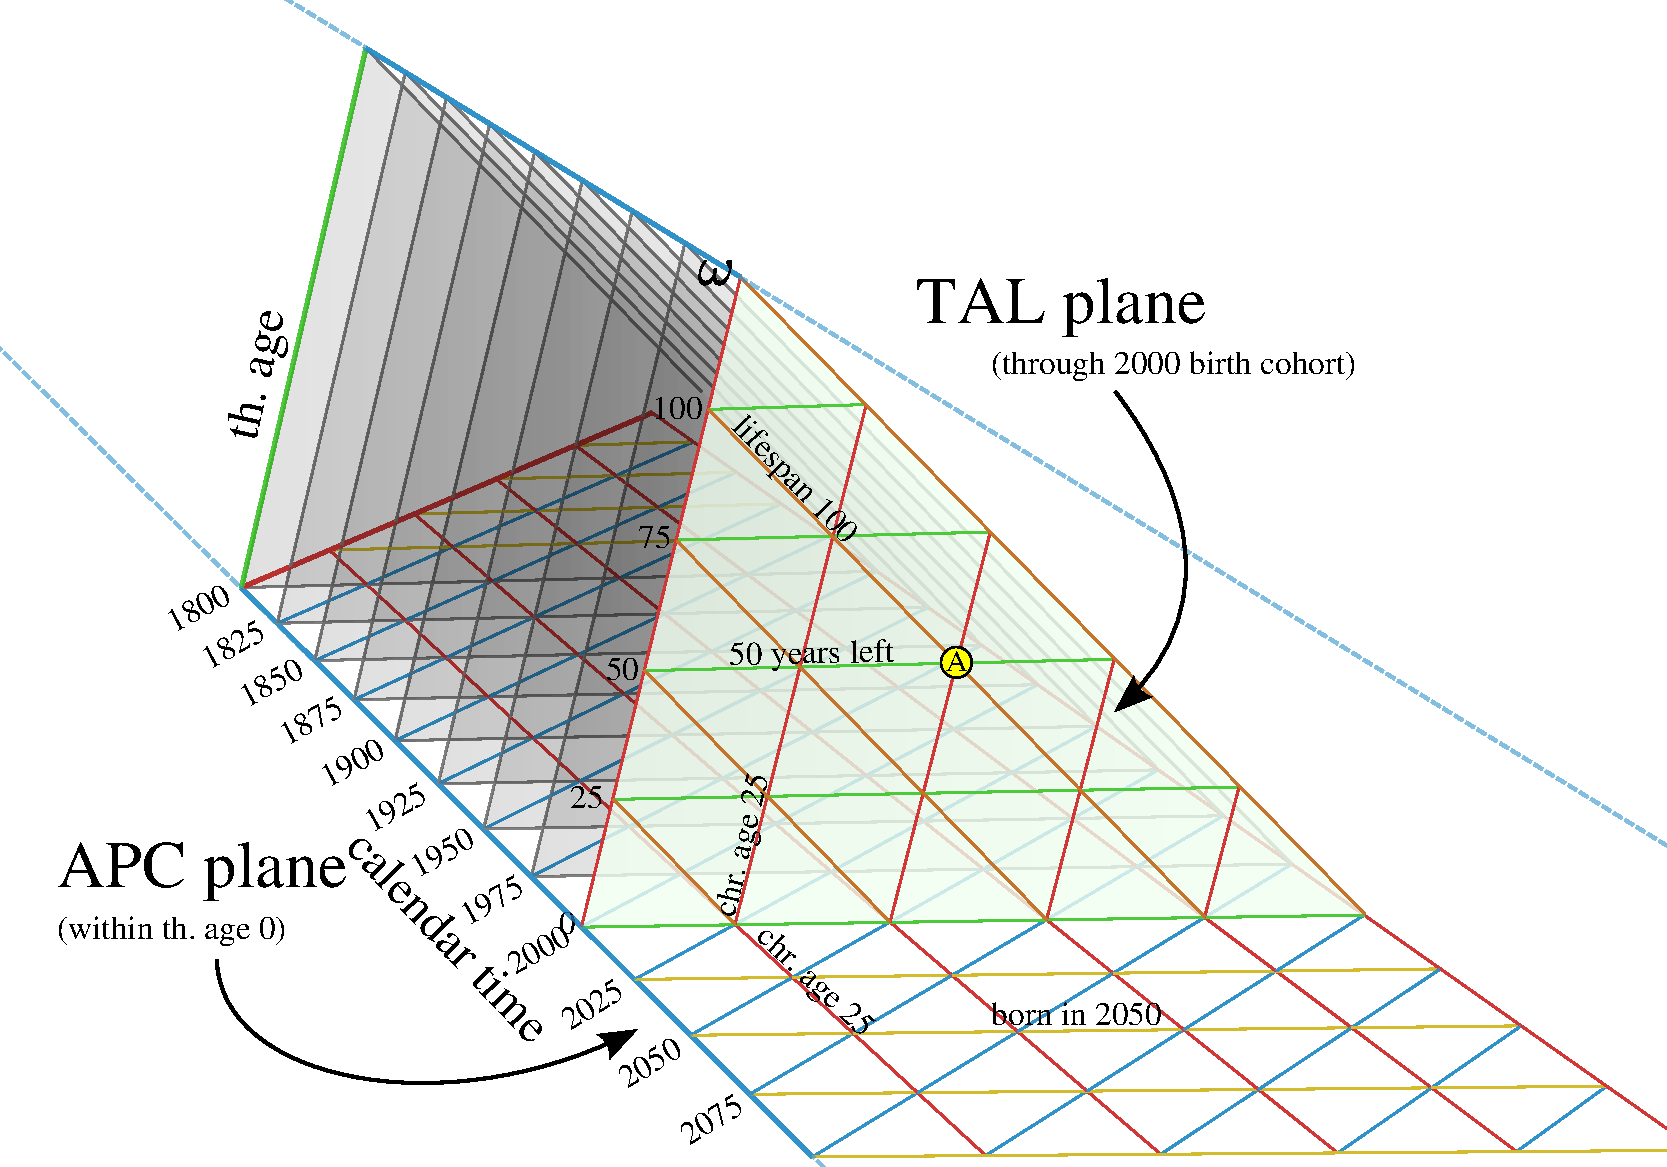
\includegraphics[scale=.5]{Figures/TALisomarkedup2.pdf}
%\end{adjustwidth}
\end{figure}

For example, imagine an infant born in the year 2000. Without further
information, we only know that this infant is located somewhere on the
thanatological age axis of the front TAL plane. If this infant is
destined to die in the year 2100, then the vertical position at birth will be at the axis tick for thanatological age 100. This
person's entire life stays on the 100 lifespan line (labelled),
descending over time towards thanatological age 0. Point A marks the midpoint in
life for this individual, at chronological age 50 (red line, labelled), and
thanatological age 50 (green line). If another APC plane were drawn through thanatological age 50, we would see that point A is in the year 2050. Since all individuals born in the year 2000 complete the same age in the same year, we can
also recuperate the year for point A by following the chronological age 50 line
(red) down to where it meets the blue line for the year 2050. The lifeline
descends downward toward the APC plane for thanatological age 0 at chronological age 100, meeting the year 2100, which determines the death cohort. 

The density and location of imaginary lifelines in this diagram, omitting
migration, is purely a function of birth cohort size and survival. For extinct
cohorts all lifelines can be positioned, but for the 2000 birth cohort this is
not yet the case. Most of the front TAL plane is in the future. One may imagine
yet another plane intersecting this space--- the ``present plane'', which is
identical to the period TAL plane for the present moment. To see how this plane
divides the space, imagine that we are in the year 2025, and follow the blue
line in the APC base inward 25 years to where it meets the red line for chronological age 25, and follow the
red line up the front TAL plane. A single plane cuts through the year
2025 and chronological age 25 from the year 2000 birth cohort. This plane
shifts forward or backward in time to meet the present year. In this particular
plane, the coordinates T, L, and D are uncertain. The period TAL plane $\omega$
years in the past is fully identified, ergo, theoretically the lifespan of each
individual in the time of Lexis is knowable. 

Fig.~\ref{fig:apctTAL} could have been drawn with TPD or LCD planes highlighted
as well, but these can still be imagined upon the current rendering. TPD planes
transect this space through any given chronological age, for instance. Imagine a
wall on the left side of the prism, cutting through chronological age 0. In this
case, the thanatological age axis is indicated in the very back of the diagram,
calendar time becomes another axis, and death cohort diagonals are not drawn.
TPD planes sequence inward from this first plane, always forming cross-sections
through chronological age. The LCD plane is to be found by rotating the current
prism such that the angle of view is directly down (or up) lifelines, which
appear as points.

Further, the two classes of planes drawn
(APC and TAL) could have been drawn and labelled differently.
In practice, the diagram of any triad identity may be drawn held constant for any one of its
three missing indices with no loss of generality. For example, we have
mentioned period (P) and birth cohort (C) TAL planes, but there must also be a
third TAL plane that is held constant for death cohort (D). Another example
of such multiplicity is found in the birth cohort TAL diagram. In this diagram,
lifespan lines can also be interpreted as death cohorts (D), chronological age
lines are also period lines (P), and thanatological age (T) is maintained. This
means that the birth cohort TAL diagram is also a birth cohort TPD diagram.
Multiplicity of this kind can be systematically confirmed, since the C time measure is not part of TPD. To not overly extend this exposition, and to avoid undue confusion, we neither delineate every possible cross-section nor the possible interpretations of each cross-section.
However, in general there are four total ways to cut the
space that are parallel to the faces of the hexad identity, and each cut
has three possible diagram interpretations.

The essential property of this perspective diagram is that lifelines
start and end in parallel, desceding downward and forward in time. A real
population of renewing lives, spread over time and over the typical range of
human lifespans, will tend to fill the entirety of the prism depicted in
Fig.~\ref{fig:apctTAL}, and any given point in the prism can be given six
demographic time coordinates, of which two or three are redundant.

%Since the APC plane at the base of Fig.~\ref{fig:apctTAL} could have been
%drawn for any thanatological age (horizontal planes at different levels), it is
%better to imagine the TAL plane slicing through the same birth cohort, $t$, of
%every possible thanatological APC plane.
%In Fig.~\ref{fig:apctAPC} we gaze from a different angle and highlight
%different planes to emphasize how the APC planes stack by thanatological age.
% The space in
%this view is capped by period TAL planes on either side. Think of period TAL
%planes as population censuses that have been fully linked to
%mortality outcomes, such that each person is categorized by thanatological
%age as well as chronological age (and each of the other indices). Period
%TAL planes shift over time, like the birth
%cohort TAL planes in Fig.~\ref{fig:apctTAL}, but the period and cohort TAL
%planes stand in intersection.

%\begin{figure}[!h]
%\centering
%\begin{adjustwidth}{-6em}{-6em}
%\caption[cap]{The APC plane of thanatological age 25, with period TAL planes.}
%\label{fig:apctAPC}
%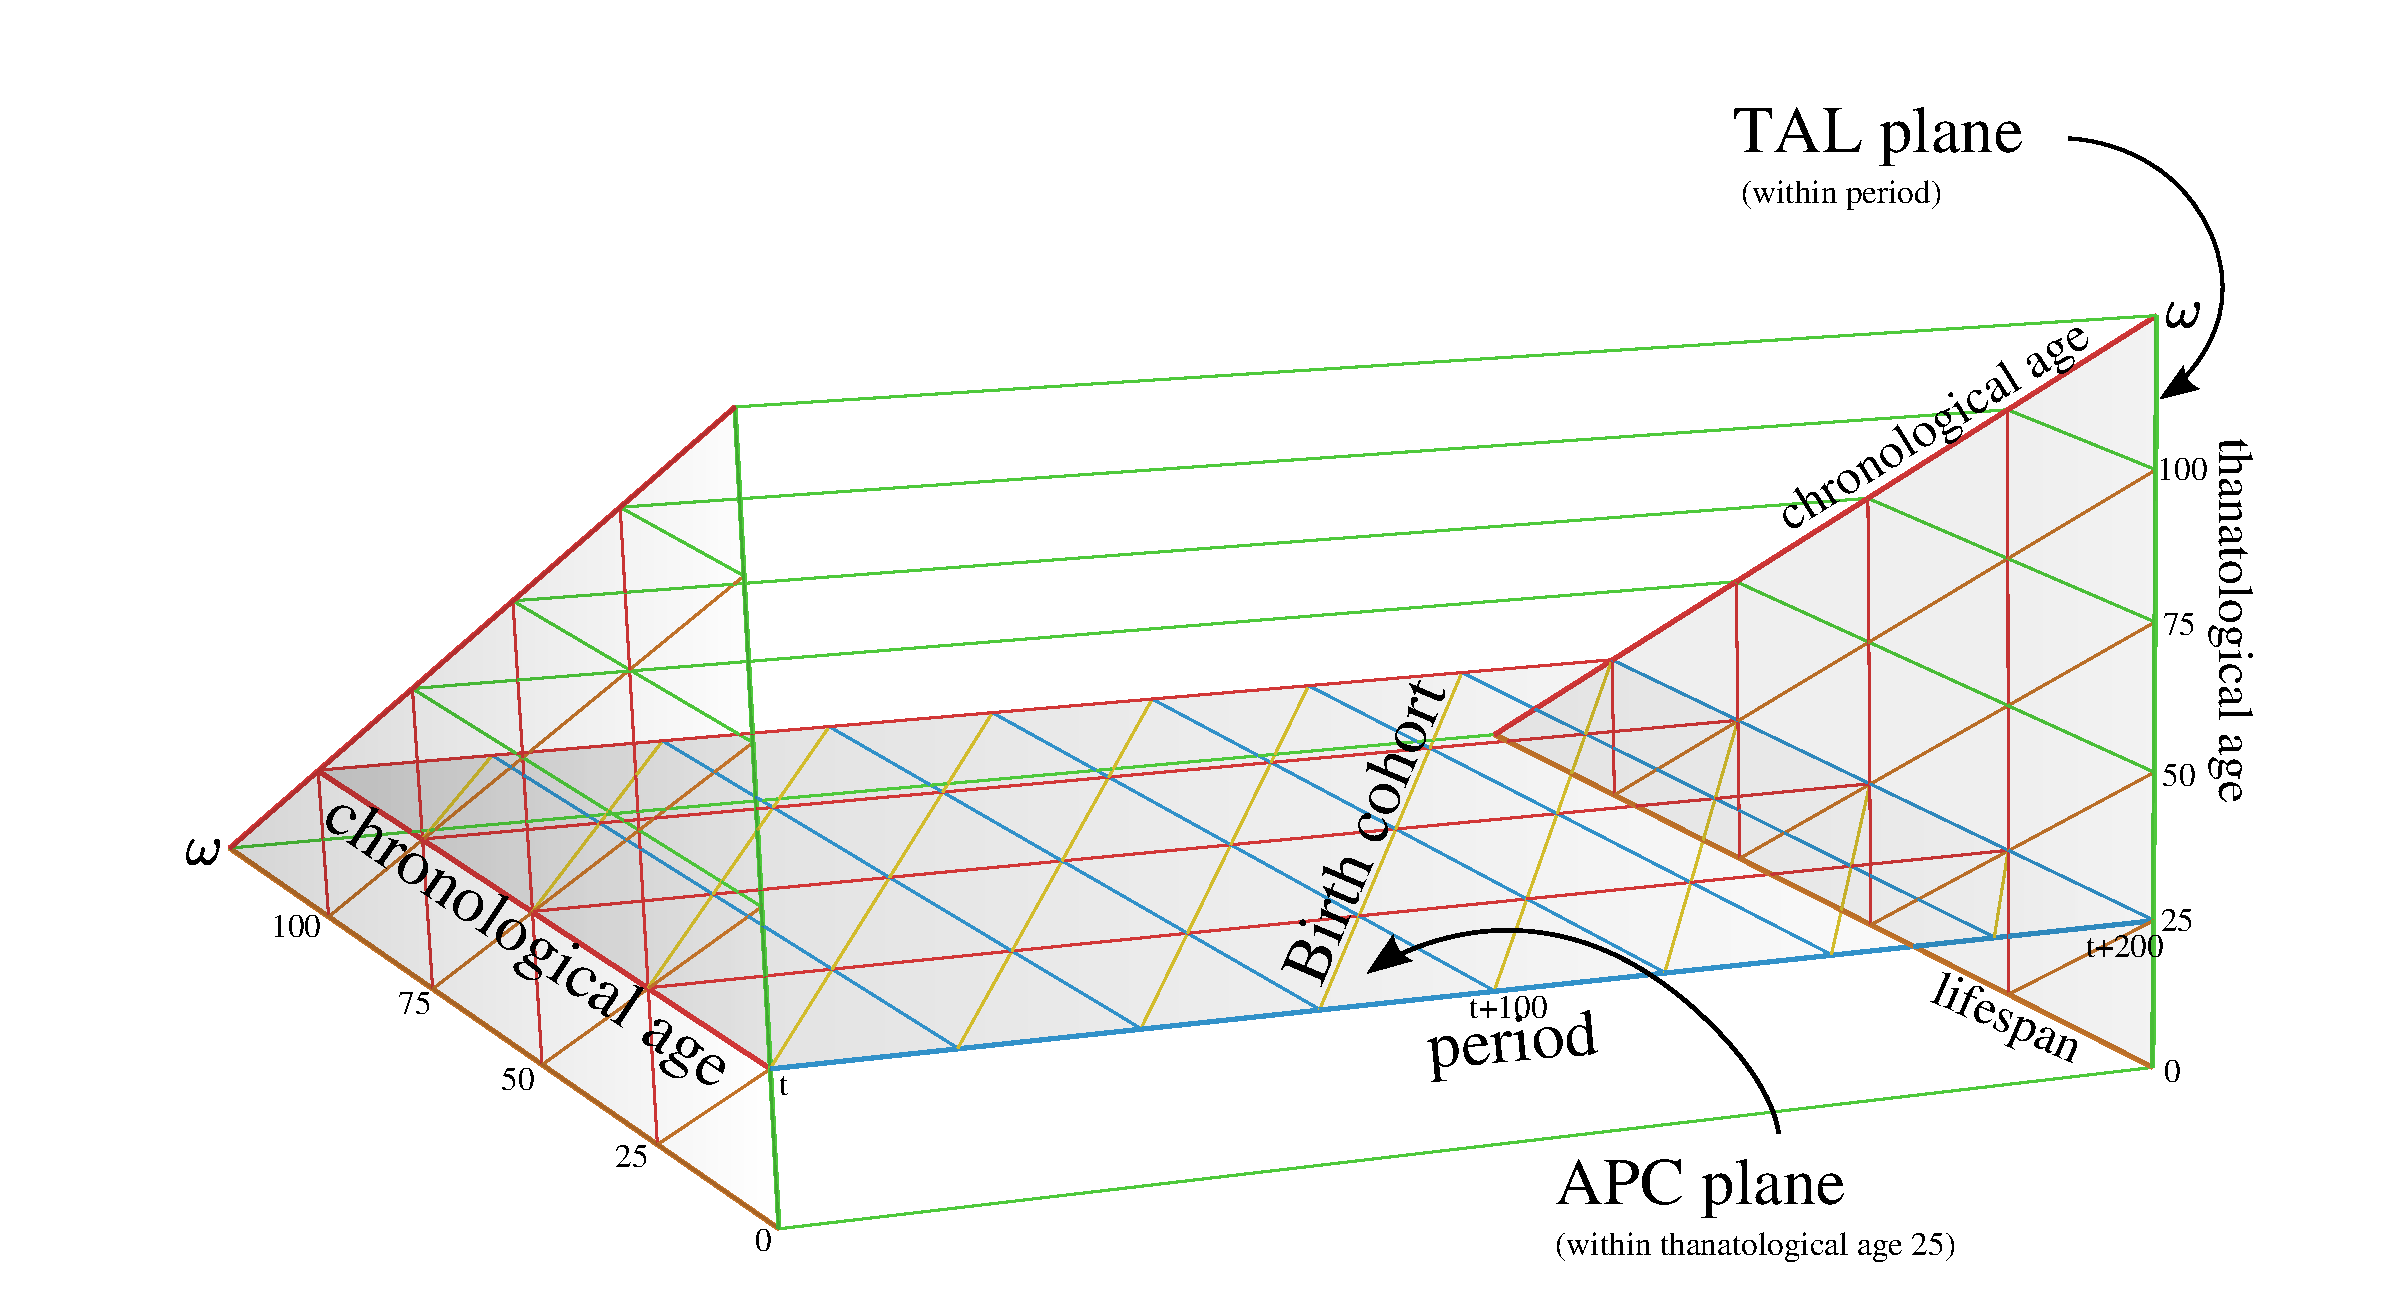
\includegraphics[scale=.5]{Figures/APCisomarkedup.pdf}
%\end{adjustwidth}
%\end{figure}

%The APC shown in Fig.~\ref{fig:apctAPC} is drawn for thanatological age 25,
%but we can think of it as shifting up and down through the space.
%At the peak, near $\omega$ remaining years of life, the age axis of the plane
% is short, since
%only the lowest chronological ages may live so long. The APC base plane at
%thanatological age 0 is the largest because members of any chronological may
%die. 

%\FloatBarrier
%\section*{Data visualization}
%The perspective renderings of the hexad identity in
%Figures~\ref{fig:apctTAL} and~\ref{fig:apctAPC} show how the four
%planes intersect and repeat to fill a space. These references help understand how the six measures of demographic
%time relate to fill a space in such a spatial construction, but this does not mean that said
%structure is necessarily the best way to visualize data. To visualize data directly in the 3d
%space would imply visual overlap, whether the data is categorical or continuous.
%We briefly discus the cases of continuous data and sequences within lifelines,
%both of which will typically lead one to produce small multiples of plots in
%order to understand the composition of demographic variables through the space.
%
%For the case of continuous information, much can be learned by looking at
%general strategies to visualize quantitative information through a 3d space (weather
%models, fMRIs, geology). Most such strategies are either fully interactive or
%represent series of cross-sections at regular intervals through the space. The
%latter choice is much easier for the researcher to implement.
%In the present case, cross-sections could be any of the four planes (triad identities) held constant for a given value of the
%dimension that is controlled for or ``sliced through''. For example, a set of
%TAL contour plots (similar to ``Lexis surfaces''), each for a different birth cohort,
%displayed as a small multiples series \citep{tufte1983visual} is one
%way to visualize data in the construct we propose. This is the strategy we follow in the application example.
%
%The familiar notion of a life line may be directly applied within the
%hexad identity without much modification. For example, would could retrofit the
%``Lexis Pencil'' instrument of \citet{francis1996visualization} to display
%multiple categorical states within individuals over the life course. The legibility of said visualization would
%be inversely proportional to the number of life lines in the plot. Life lines are useful for small
%sets of individuals and for demonstrative purposes.
%
%A set of cohort life lines squeezed together and sorted by lifespan becomes a
%survival curve. Event charts \citep{goldman1992eventcharts,lee2000extensions}, or
%visually richer event history graphs \citep{carey1998simple,dubin2001event} have
%been developed as a way to display within-individual sequences inside survival
%curves. Such plots in our framework would also necessarily apply to the birth
%cohort TAL slice, and would probably need to be displayed in small multiples.
%For large numbers of life sequences, one may apply some version of the
%grouping or smoothing techniques proposed by \citet{piccarreta2012graphical} or
%\citet{fasang2013visualizing} in order to reduce noise. 
%
%For both the case of visualizing continuous variables or sequences within
%lifelines, individuals that are censored because they are not yet dead (and therefore only
%have three known time measures) cannot be fully situated in this framework.
%Assigning living individuals death times is a larger
%statistical question about the prediction of remaining lifetime for living
%individuals, and it is neither a problem peculiar to the present case of
%visualization nor .
%One can either opt to omit living individuals from the 3d space, as their
%coordinates are not yet determined. This is the course we take in the application example. Often one would like to predict for censored individuals, either for the sake of making a more
%relevant statement about an entire population stock \citep{wolf2015disability},
%or for the sake of completing an event history graph so
%as to better communicate a distribution \citep{dubin2001event}. In this case the
%modeling choice for imputing remaining lifetime is a separate question beyond
%the present treatment. Imputing remaining lifetime necessarily
%expands the bounds of the framework into the future, so as to contain the
%imputed individuals. The outer bounds of the framework are already
%determined, as they are purely a function of the maximum attainable lifespan, if
%there is such a thing.
%

\FloatBarrier

\section*{Application}
The relationship between the six measures of demographic time is true in the
same sense that mathematics is true: Under linear time it is an internally valid
set of relationships, and this is self-evident. We have mentioned that the
coordinates described here may be useful for the visualization of data, to
enable discovery, and to better inform demographic methods. We have not yet
mentioned how such developments might arise in practice. We therefore give a
schematic overview of our own process of scientific inquiry and reflection that was based this coordinate system, and
that would not have arisen without it. This chain of inquiry is meant to demonstrate the
usefulness of the present framework, but it is far from an exhaustive
application of its potential for other substantive questions, nor is the case
study described in complete rigor. Specifically, we reason that
projections or comparisons of healthy life expectancy (HLE) are in many
cases biased in period prevalence-based models unless one takes into account the
thanatological age pattern of prevalence, as well as mortality differences.

There are three steps in our empirical inquiry. The first step is to visualize
variables on health outcomes using our framework. The second step is to
assess the primary time measures over which health outcomes appear to vary.
Under the assumption that these patterns of temporal variation are empirically regular,
we proceed to develop a method of standardizing health expectancy calculations
for morbidity conditions whose prevalence is more closely related
to thanatological age.
Finally, one can reason that period estimates of health expectancies for certain
health conditions are biased when mortality has been or will-be changing, and
comparisons of HLE between populations with different mortality are also biased.
We conclude that comparisons of health expectancies might be biased in ways not
previously documented.

Let us take the example of self-reported health (SRH). This variable is
available from many different survey sources, and it is familiar to many researchers. There are
many known pitfalls to this particular variable that already make it difficult
to compare between sexes, over time, or between populations, and these do not
concern us. We use this variable as an example because of the clear
pattern of variation that it shows, which we use to make our more general point.

Figure~\ref{fig:poorsrh} displays a series of TAL surface plots, each referring
to a different quinquennial birth cohort (1905-1909, etc). The data come from
the RAND version of the US Health and Retirement Study \citep{HRS}. Since this
survey has multiple observations of individuals, as well as a mortality
follow-up, we have each of the six time measures for each observation. Further methodological details are given by \citet{riffe2015ttd}. The TAL surfaces for each birth
cohort are shifted by five years because the observation window available is
from 1992 to 2011 for each cohort.

\begin{figure}[h!] 
\caption{Prevalence of males self-reporting poor health by chronological and
thanatological age, by quinquennial birth cohorts, 1905-1925. (HRS)}
\label{fig:poorsrh}
\centering
\vspace{-1em}
\begin{subfigure}{.46\textwidth}
\centering
\caption{1905}
\vspace{-1em}
\label{fig:srh1905}
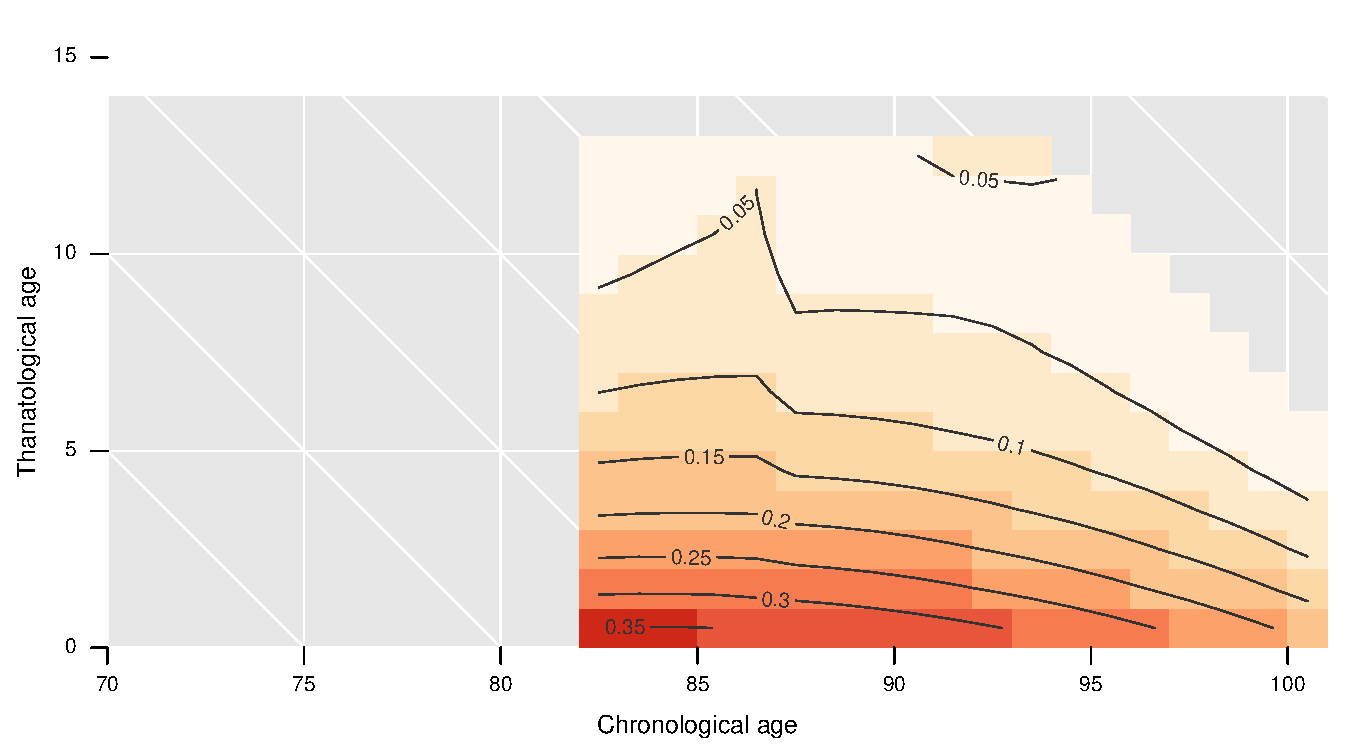
\includegraphics[scale=0.32]{Figures/TALapplication/srhpoor1905.pdf}
\end{subfigure}
~
\begin{subfigure}{.46\textwidth}
\centering
\caption{1910}
\vspace{-1em}
\label{fig:srh1910}
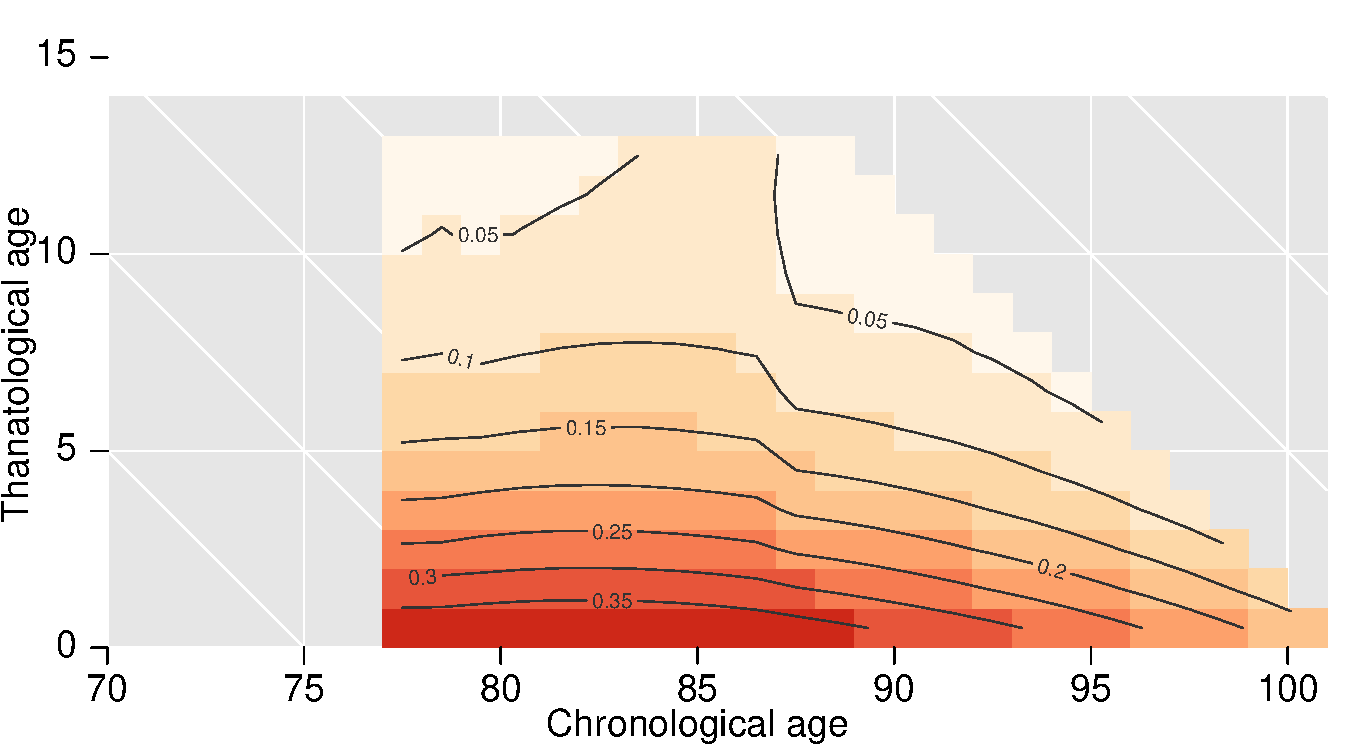
\includegraphics[scale=0.32]{Figures/TALapplication/srhpoor1910.pdf}
\end{subfigure}

\begin{subfigure}{.46\textwidth}
\centering
\caption{1915}
\vspace{-1em}
\label{fig:srh1915}
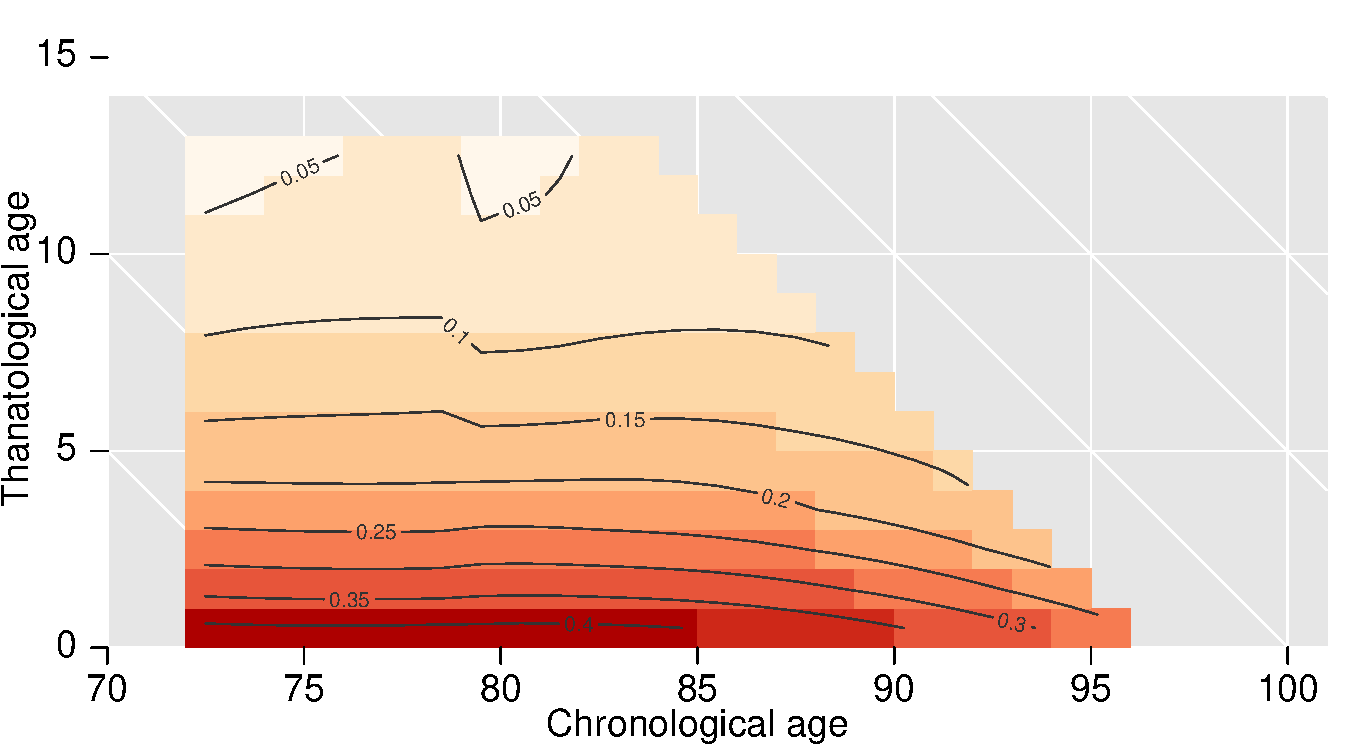
\includegraphics[scale=0.32]{Figures/TALapplication/srhpoor1915.pdf}
\end{subfigure}
~
\begin{subfigure}{.46\textwidth}
\centering
\caption{1920}
\vspace{-1em}
\label{fig:srh1920}
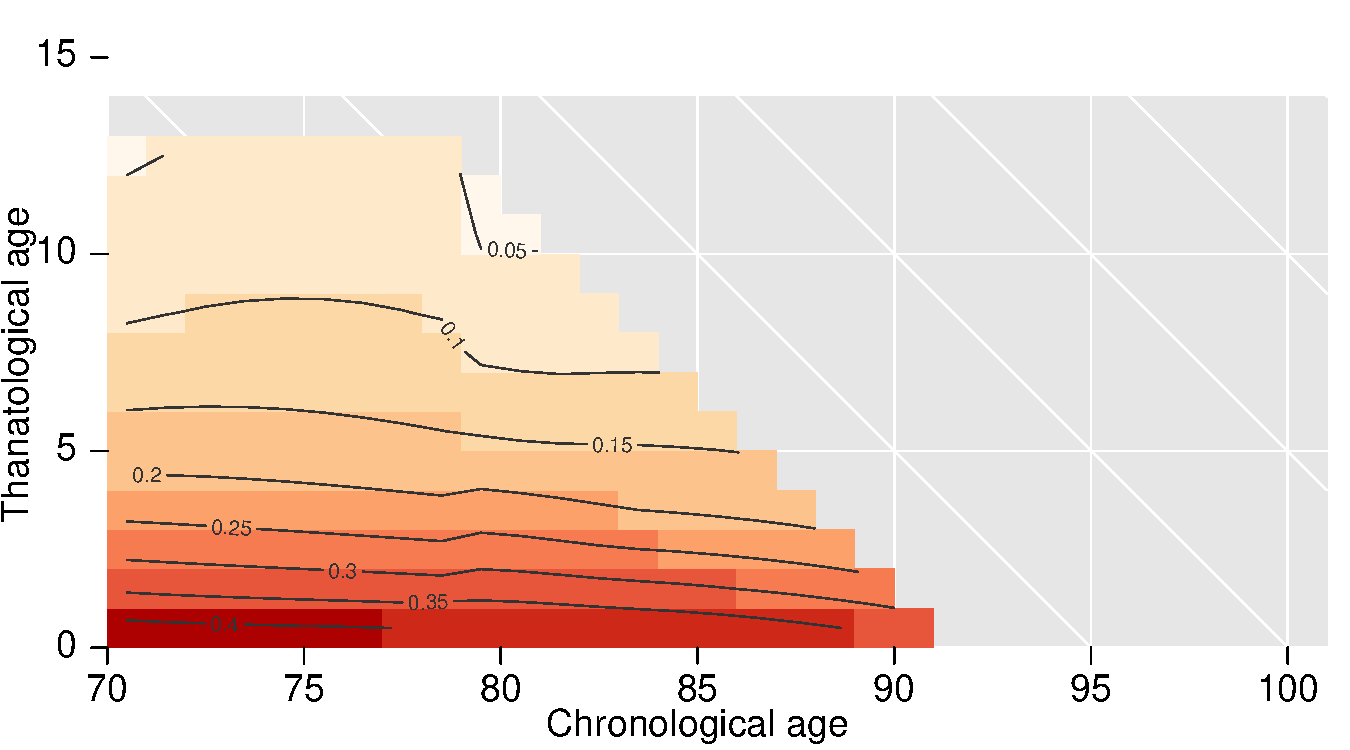
\includegraphics[scale=0.32]{Figures/TALapplication/srhpoor1920.pdf}
\end{subfigure}

\begin{subfigure}{.46\textwidth}
\centering
\caption{1925}
\vspace{-1em}
\label{fig:srh1925}
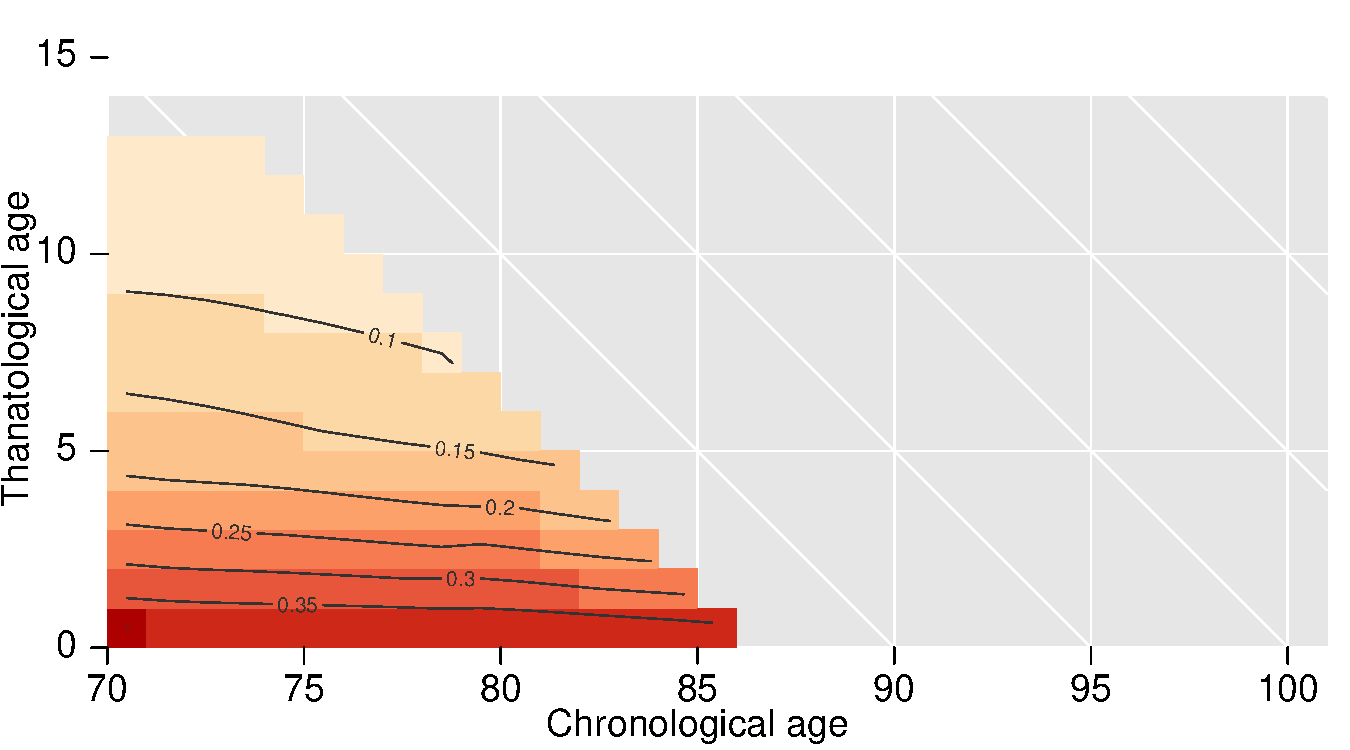
\includegraphics[scale=0.32]{Figures/TALapplication/srhpoor1925.pdf}
\end{subfigure}
~
\begin{subfigure}{.46\textwidth}
\centering
\caption*{~}
\vspace{-1em}
\label{fig:srhlegend}
\includegraphics[scale=0.32]{Figures/TALapplication/Legend.pdf}
\end{subfigure}
\end{figure} 

The $x$-axis of these surface plots is chronological age, while the $y$-axis is
remaining years of life. Contour lines in the surfaces indicate the
primary direction of variation, in this case over thanatological age. Downward
diagonals indicate lifespans, which the reader may also think of as very
specific birth-death cohorts. These are the diagonals along which lifelines may
be imagined, as suggested in Figs.~\ref{fig:TAL} and~\ref{fig:apctTAL}. For each
of these birth-death cohorts we have a prevalence trajectory--- empirical examples of the lifeline morbidity trajectories often conceptually diagrammed in the literature on morbidity compression
\citep[e.g.,][]{fries2005frailty}.
In each surface the primary direction of variation is along thanatological age,
and not chronological age. The prevalence for those with $t$ remaining years of
life is similar in these data, irrespective of chronological age, birth cohort,
or ultimate lifespan.

When one looks at a chronological age pattern of SRH, as measured
here (the Sullivan curve, \citep{Sullivan1970}), one sees an increasing tendency
over age.
However, such an increasing line is a marginal ruse, due to an interaction
between the distribution of lifespans and the relatively fixed underlying
pattern of morbidity seen in Figure~\ref{fig:poorsrh}. These surfaces can indeed
be tidily summarized with a single line, but it is a line over the
thanatological age margin rather than over chronological age. 

Since the patterns for each of these cohorts can be presumed to be the same, any
shifting in the distribution of lifespan ought not produce a change in the
expected years of poor health for a given lifespan. Further, the life years
spent in poor health should also be approximately the same ``on average'', even
if the underlying mortality patterns shift. If morbidity change is a pure
function of thanatological age, an increase in life expectancy should increase
healthy life expectancy by the same amount. This is not the prediction when we
base analyses on the chronological age pattern of self-reported health. An
underlying morbidity pattern this stable would predict improvements in the
marginal chronological age pattern of self-reported health if the lifespan
distribution were to shift right. This bias in the current status quo of
morbidity measurement and prediction leads to pessimistic morbidity scenarios
when mortality improvements are foreseen, and it undermines health expectancy
comparisons between groups with different mortality. Cohort health expectancies
are in either case unbiased, but these are also not common.

Using the data from our example surfaces, we can calculate an average prevalence
trajectory with the approach to death and calculate some basic results that
support our case. Let us take the population of US males aged 60 and older, and
assume that the trajectory derived from the Figure~\ref{fig:poorsrh} surfaces
is valid for them.
If we apply this trajectory to the synthetic stationary population of each
year from 1980 and 2010 \citep{HMD}, we can calculate the resulting healthy and
unhealthy life expectancies, and compare these with the expectancies that we would have projected assuming the 1980 Sullivan curve.
Total remaining life expectancy at age 60 increased 4.3 years from 17.4 to 21.7
years from 1980 to 2010. Assuming the thanatological trajectory of
morbidity, we calculate healthy life expectancies of 15.7 and 19.9,
respectively, an increase of 4.2 years. Unhealthy life expectancy in this
scenario increased just 0.1 years. Had we used the Sullivan curve from 1980 to
calculate the 2010 values, we would have predicted an increase of 0.7 years in
unhealthy life expectancy, or 39\% versus the 4\% ``observed'' in this
exercise.

This is a large difference in projected morbidity, and it is based on a
relatively minor tweak to standard methodology, itself inspired by viewing data under the conditions
enabled by this temporal framework and adjusting standard demographic methods
to capture the direction of temporal variation in data. There is a wide variety
of prevalence patterns when viewed in this way \citep{riffe2015ttd,
wolf2015disability}, and much empirical and methodological work is still required to verify
these findings and understand the consequences for the standard ways of
comparing and projecting HLE. Our objective in this application has been
to demonstrate how viewing data under the rigorous conditions enabled by the
time-framework we propose can lead to new scientific understandings of
processes over the life course.

%In Lexis-nomenclature, the 3d projections of an AP square, and AC or PC
%parallelograms are all congruent shapes known as regular trigonal trapezohedra
%(RTT). The orientation
%of a given RTT uniquely defines the Lexis shape in question. Similar constructs
%exist in the other time dimensions. 

%This three
%dimensional space is not only useful for the sake of formalizing observed
% temporal relationships, but also for enclosing demographic time in the past and future (e.g., before the first census and after the most recent census).

%\texttt{formerly the subsection ``Intersecting planes''. Now needs to work into
%discussion.}

%The APC, TPD, TAL, and CDL planes can be conceived of either as
%\textit{compressions} of this 3d space, or as cross-sections of the 3d space.
% To compress space in this sense is to ignore the missing dimension,
%whereas a cross-section sets a given triad identity against a particular
%position of the absent dimension. This is a more general sense of the term
%\textit{cross-section} than is often used in the demographic literature, where
%it typically implies a period cross-section.
%APC has thus far always been treated as a compression in this sense.
%As mentioned, a compressed TPD diagram has thus far only appeared
%in \citet{villavicencioRiffeSymmetires2016}, and cross-sectional TAL diagrams and surfaces have thus
%far only appeared in \citet{riffe2015ttd}. 
%. This TAL usage was selected for the 1915-1919 birth
% cohort, and therefore belongs to the 3d space,
 % \raisebox{-.25\height}{\includegraphics[scale=.15]{Figures/triadtable/ATLC.pdf}}.
%We have been unable to locate an example in the literature of a
% compressed TAL or cross-sectional TPD diagrams, though it seems plausible that
 % the former will have arisen. We suppose
%that LCD diagrams of any kind are novel. 


%either as a visual
%diagnostic or in any line of inquiry or argumentation.
%\footnote{There are, however, some novel temporal
%juxtapositions in the literature on event analysis of
%big data \citep[see e.g.,][]{watson2015timemaps}.}

\FloatBarrier
\section*{Discussion}

It is straightforward to
think of examples to derive time measures based on other given
time measures. In isolation, the various triad identities are also intuitive.
The TPD diagram is similar to APC, but it is aligned to time of death rather
than time of birth. The TAL diagram presents a clear way to classify events
over the life course of a cohort. Finally, the LCD diagram can be used to
structure quantities that vary over time and by length of life.
Joined together, the relationship between all six time measures is more
complex than any of the triad identities, but it condenses into a simple
geometric representation that can be easily derived by ascribing the various time measures to the six edges of a tetrahedron. An understanding of how the six time measures relate is
key to understanding the temporal structure of demographic processes, which
itself underlies the comparability of demographic measures.

A simultaneous juxtaposition of
the six demographic time measures has never appeared in the literature. However,
\citet{lexis1875einleitung} describes an analogous hexad relationship between,
birth cohort, age at marriage, age at separation (death or widowhood), marriage cohort, separation cohort, and
duration of marriage. The hexad relationship between these six
time measures can also be verified on a tetrahedron graph. Lexis also describes
cross-sections in the same sense (\textit{Schnitte}) that we do, denoting
two-dimensional diagrams, with values of the orthogonal dimension held constant.
This identity is coherent, but it does not find perfect
analogy in our proposed framework, in part because each lifeline in the Lexis
hexad identity has up to three possible points. The period dimension is
not explicit, but rather nested within three varieties of cohort.
Clearly with age, \textit{period}, and total duration, remaining
time should also be identifiable, but this is not included in Lexis' hexad
identity. Our hexad identity is designed to contain and identify any point on
the lifecourse of individuals in populations with heterogeneous
lifespans. As such it fully describes a population of single state durations.
We liken the Lexis identity to something similar to a two state APC, albeit
without explict period. We do not claim that the concepts in Lexis' hexad
identity are not transportable, but perhaps the specificity of this identity has made it unwieldy in practice, or difficult to conform with data.

The contemporary practice of (macro) demography is based on the premise that
vital rates, and other kinds of rates over the lifecourse, are the truest measure of
demographic forces. Rates are paramount because they tend to vary in
empirically regular ways over the life course. The scalings and movements of
primary vital rates fall within a limited range for humans. For this reason, many of the methods of
demography are developed to estimate rates, independent of population composition, or to
partition crude magnitudes into the effects of population age structure and
pure vital rates. Controlling for age is in a more general sense controlling for
temporal variation in stocks. To the extent that regular temporal variation
relates to the end of life, or the length of life, common
age-standardization does not fully account for such structure.

The techniques used to age-standardize mortality and fertility estimation are at
times applied to other kinds of transitions over the life course. For example,
one may estimate an age pattern to some degenerative disease, or the
ability to carry out some common activities of daily life. Much of the
regular temporal variation for such conditions is by time-to-death or
lifespan, rather than by chronological age. Apparent chronological age patterns
for such conditions are artifactual and do not represent the same kind of
intrinsic meaning as does the \textit{age pattern} of mortality. Further kinds
of temporal standardization must be developed in order to measure and understand
the natural patterns of such conditions over the lifecourse. 
The measurement of
such conditions may benefit from consideration of the framework presented in
this paper. To this end, Table~\ref{tab:set3} provides all combinations of
information that are sufficient to derive the full set of six time measures.
Panel surveys with mortality followups already provide the requisite
information, as do linkable registers that include items such as
health measures or proxies and relevant dates of birth, observation, and death.

The best way to seek regular patterns in variation
is via data visualization. The coordinate system proposed in this paper is
conceived as one adequate to capture all such variation, and we suggest its use
for visualizing data, probably via small multiples of successive time slices
parallel to any of the four triad identities, similar to that shown in
Figure~\ref{fig:poorsrh}.
Such visualization strategies at this time are exploratory, and this is a
technique that may benefit from further refinement. 

The 3d diagram of the hexad identity we propose is reminiscent of some rigorous
descriptions found starting in section IV of \citet{lexis1875einleitung}. Lexis
provides a rigorous treatment of the hexad identity between birth cohort ($n$), age at
marriage ($\alpha$), age at separation due to death or widowhood ($a$), marriage cohort ($\chi$),
separation cohort ($z$) and duration of marriage ($\delta$). He also slices
through this hexad space to produce cross-sections that also find direct
parallels in our triad identities. The marriage hexad identity is also
illustrated with complex perspective line drawings (see Lexis' Figures 5 and 6).
These figures (based on cubes rather than tetrahedra--octahedra) and the portion of
the text that discusses these relationships has unfortunately been largely
overlooked in posterior literature, which has focused much more on the APC
plane. We are fortunate to have noticed it in the course of this work, not least
because Lexis' use of marriage durations is itself a good example of the
translation of the demographic time framework used in an event history setting.
This further highlights the fact that we are in a general sense simply modeling sets of durations of variable length that are distributed over time. 

Our hexad diagram is also reminiscent of the Lexis pencil notion from
\citet{francis1996visualization}. That visualization system could be
constrained to match the one we present if the $z$ axis were set to remaining
years of life and lifeline trajectories were realigned to descend toward zero remaining years of life (or some rotation thereof).

Mortality determines three of the dimensions of
demographic time, and it therefore makes little sense to model mortality using
all six time measures. Any of the six measures may be pertinent in the case of
conditions and states that vary over and within the lifecourse. The most obvious application
for the present model, given data commonly (and publicly) available at this
time, are late-life health conditions, although there may be other substantive
areas of application. 

Furthermore, we believe in the pedagogical value of the framework
introduced in this paper. We hope that the
present inquiry will be useful as a teaching instrument in the same way as APC
diagrams have formed a part of basic demographic education.
The relationship between the six dimensions of demographic time helps situate the APC
paradigm in a broader framework. Just as scientific discovery in general
depends partly on the development of finer optics and instrumentation, we hope
that the framework we give will be an instrument to enable new discoveries
in formal and empirical demography.


% remove appendix, it pushes figures + tables past 10\ldots
%FloatBarrier

%\begin{appendices}
%\section{Variants of tetrahedron graph}
%The graph depicted in Figure~\ref{fig:tet} could be drawn with any of the
%four vertices in the middle of the triangle (as well as other inversions
%and rotations).
%These would all serve equally well to present the same aspects of the model,
% and we have no insight as to whether one of these renditions is more or less
%intuitive. Figure~\ref{fig:app:tet} provides four perspectives on the
%tetrahedron, for the case that this aids in understanding. The reader may make
% a paper tetrahedron, with labeled edges and vertices to be convinced that
%these are identical graphs.
%\begin{figure*}
%        \centering
%        \caption{Some variants of the graph of the APCTDL tetrahedron.} 
%         \label{fig:app:tet}
%        \begin{subfigure}[b]{0.475\textwidth}
%            \centering
%            \includegraphics[width=\textwidth]{Figures/Tetra1.pdf}
%           \caption{\small Vertex \vt{1} in middle. APC Northwest.}
%            \label{fig:tet1}
%        \end{subfigure}
%    \hfill
%        \begin{subfigure}[b]{0.475\textwidth}  
%            \centering 
%            \includegraphics[width=\textwidth]{Figures/Tetra2.pdf}
%           \caption{\small Vertex \vt{2} in middle. APC Northeast.}
%            \label{fig:tet2}
%        \end{subfigure}
%        \vskip\baselineskip
%        \begin{subfigure}[b]{0.475\textwidth}   
%            \centering 
%            \includegraphics[width=\textwidth]{Figures/Tetra3.pdf}
%           \caption{\small Vertex \vt{3} in middle. APC Northwest.}
%            \label{fig:tet3}
%        \end{subfigure}
%        \quad
%        \begin{subfigure}[b]{0.475\textwidth}   
%            \centering 
%            \includegraphics[width=\textwidth]{Figures/Tetra4.pdf}
%            \caption{\small Vertex \vt{4} in middle, as in
%            Figure~\ref{fig:tet}. APC base.}
%            \label{fig:tet4}
%        \end{subfigure}
%    \end{figure*}
%\end{appendices}
%%FloatBarrier

\bibliographystyle{chicago} % required for demography
%\bibliographystyle{plainnat}
  \bibliography{references} 

\end{document}